% !TeX spellcheck = en_US
\documentclass[12pt]{article}

\usepackage{times,fullpage,xspace,fancyhdr,url,color}
\usepackage[pdftex]{graphicx}
\usepackage[pdftex,
            colorlinks=true,
            urlcolor=black,
            linkcolor=black,
            citecolor=black,
            bookmarksopen=false,
            bookmarksnumbered=true,
            pdfstartview=FitH]{hyperref}

\pdfcompresslevel=9
\newcommand{\leaguename}{RoboCup Standard Platform League (NAO) }
\hypersetup{
 pdftitle={\leaguename Rule Book},
 pdfauthor={Technical Committee SPL},
}
\usepackage{microtype}
\usepackage[utf8]{inputenc}
\usepackage{amsmath}
\usepackage{xargs}
\usepackage[colorinlistoftodos,prependcaption,textsize=tiny]{todonotes}
\usepackage{siunitx}
\usepackage[capitalize,noabbrev]{cleveref}
\usepackage[official]{eurosym}
\usepackage[useregional]{datetime2}
\usepackage{subcaption}
\usepackage{enumitem}
\usepackage{xcolor}
\DTMlangsetup[en-GB]{ord=raise,monthyearsep={,\space}}

\newcommandx{\unsure}[2][1=]{\todo[linecolor=red,backgroundcolor=red!25,bordercolor=red,#1]{#2}}
\newcommandx{\change}[2][1=]{\todo[linecolor=blue,backgroundcolor=blue!25,bordercolor=blue,#1]{#2}}
\newcommandx{\info}[2][1=]{\todo[linecolor=green,backgroundcolor=green!25,bordercolor=green,#1]{#2}}
\newcommandx{\improvement}[2][1=]{\todo[linecolor=Plum,backgroundcolor=Plum!25,bordercolor=Plum,#1]{#2}}

% comment 'disable' in to disable all the todo notes :)
\usepackage
[
%disable
]{todonotes}

\usepackage[theorems]{tcolorbox}
\newtcbtheorem[number within=section]{hintbox}{}%
{colback=red!10,colframe=red!45!black,fonttitle=\bfseries}{th}

% !TeX root = ../SPL-Rules.tex
% !TeX spellcheck = en_US
\newcommand{\TotalWidth}{7.4}
\newcommand{\TotalLength}{10.4}
\newcommand{\GoalScoredDelay}{15}
\newcommand{\KickOffAutoTime}{45}
\newcommand{\KickOffBallFreeTime}{10}
\newcommand{\FreeKickTime}{30}
\newcommand{\FreeKickRadius}{0.75}
\newcommand{\VisualSignalTime}{2}
\newcommand{\ReadyDelayTimeChampion}{45}
\newcommand{\ReadyDelayTimeChallenge}{40}
\newcommand{\PlayingDelayTime}{15}
\newcommand{\PenaltyKickTime}{30}
\newcommand{\PenaltyKickSetupTime}{30}
\newcommand{\PenaltyShootoutKickTime}{30}
\newcommand{\StandardPenaltyTime}{45}
\newcommand{\StandardPenaltyIncrease}{10}
\newcommand{\NovelContributionTime}{3 years\xspace}
\newcommand{\GameStuckTime}{30}
\newcommand{\TeamMessageSize}{128}
\newcommand{\TeamMessageLimit}{1200} % Limit of number of packets available to one team during a game with two halves of 10 minutes.
\newcommand{\TeamMessageLimitMinute}{60} % Limit for the average number of packets available to one team during a minute of gameplay.
\newcommand{\MaxJerseyNumber}{20} % the highest allowed jersey number to wear by robot players

% !TeX root = ../SPL-Rules.tex
% !TeX spellcheck = en_US
\newcommand{\LastRCYear}{2022\xspace}
\newcommand{\RCYear}{2023\xspace}
\newcommand{\JerseyApproveSubmissionDate}{2023-05-01}
\newcommand{\CodeReleaseAnnouncementDate}{2023-10-15}


\sloppy
\newcommand{\ie}{\mbox{i.\,e.}\xspace}
\newcommand{\eg}{\mbox{e.\,g.}\xspace}
%\newcommand{\cf}{\mbox{cf.}\xspace}
\newcommand{\cf}{see\xspace}
% \newcommand{\comment}[1]{\marginpar{\pdfannot width 4in height .5in depth 8pt {/Subtype /Text /Contents (#1)}}}
\newcommand{\inparagraph}[1]{\paragraph{#1\hspace{-1em} }}


% some colors
\definecolor{orange}{rgb}{1,0.5,0}
\definecolor{red}{rgb}{1,0,0}
\definecolor{green}{rgb}{0,1,0}


\title{\leaguename Rule Book}
\author{RoboCup Technical Committee}
\date{(DRAFT \RCYear rules, as of \today)}

\setlength{\parindent}{0pt}
\setlength{\parskip}{12pt plus 6pt minus 3 pt}
\setcounter{tocdepth}{1}
\widowpenalty=10000
\clubpenalty=10000

\pagestyle{fancy}
\lhead{}
\chead{}
\rhead{}
\lfoot{}
\cfoot{}
\rfoot{}

\renewcommand{\headrulewidth}{0.4pt}
\renewcommand{\footrulewidth}{0.4pt}

% needed to align an image and text correctly side by side
\newcommand{\imagebox}[1]{\raisebox{2ex}{\raisebox{-\height}{#1}}}

\begin{document}

\maketitle

\begin{center}
  Questions or comments on these rules should be submitted via \url{https://github.com/RoboCup-SPL/Rules/issues}, to the \texttt{\#rule-book} channel on the SPL Discord server, or by mail to \url{rc-spl-tc@lists.robocup.org}.
\end{center}

\newpage

\tableofcontents
\setcounter{tocdepth}{3}

\thispagestyle{fancy}

\clearpage

\cfoot{\thepage}
\setcounter{page}{1}

\newpage

% !TeX root = ../SPL-Rules.tex
% !TeX spellcheck = en_US
\section{Setup of the Environment}
\label{sec:setup_environment}

\subsection{Field Construction}
\label{sec:field_dim}

The standard soccer field consists of \qty{8}{\milli\metre} artificial turf mounted on a flat wooden base with a total area of length~\qty{\TotalLength}{\metre} and width~\qty{\TotalWidth}{\metre}. Care should be taken to ensure the field is as flat and level as possible. Additionally, the wooden base should be well-supported and should not give when humans stand or walk on it.

\Cref{fig:field_dim} shows the dimensions of a standard soccer field.
A more detailed technical drawing is provided in \cref{apx:technical-drawing} to this document.
Note that the penalty mark is a cross and there is a dash at the midpoint of the halfway line. White field lines can be made of the same \qty{8}{\milli\metre} artificial turf, but in white (\ie, made of white artificial turf), spray-painted or taped. Regardless of the solution, the field lines must be durable throughout the competition.

\Cref{fig:goal_dimensions} and \cref{fig:goal_appearance} depict the construction and placement of the goals. A support structure for the net shall be made with small black, white, or gray bars or cylinders.  The support structure shall be constructed exactly as shown in \cref{fig:goal_appearance}.

\begin{figure}[b!]
\centering
\centerline{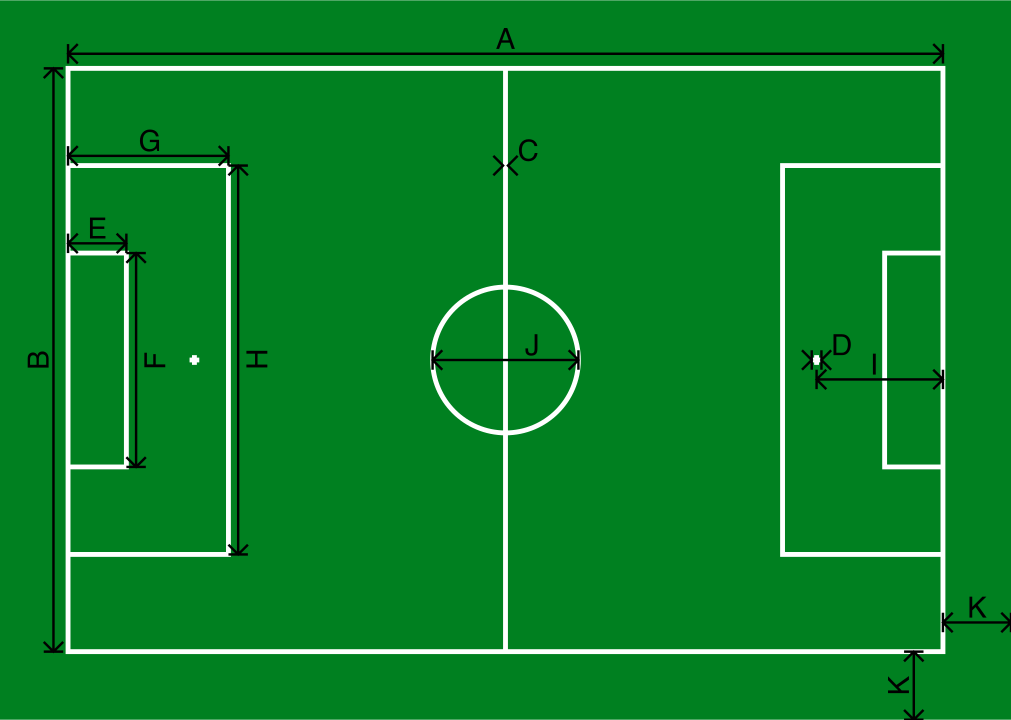
\includegraphics[width=\columnwidth]{figs/field_simple.pdf}}
\vspace{1ex}
\begin{tabular}{| l | l | l |}
ID & Description & Length (in mm) \\
\hline \hline
A & Field length & 9000 \\
\hline
B & Field width & 6000 \\
\hline
C & Line width & 50 \\
\hline
D & Penalty mark size & 100 \\
\hline
E & Goal area length & 600 \\
\hline
F & Goal area width & 2200 \\
\end{tabular}
\begin{tabular}{|l|l|l|}
ID & Description & Length (in mm) \\
\hline \hline
G & Penalty area length & 1650 \\
\hline
H & Penalty area width & 4000 \\
\hline
I & Penalty mark distance & 1300 \\
\hline
J & Center circle diameter & 1500 \\
\hline
K & Border strip width & 700 \\
\hline
 &  &  \\
\end{tabular}
\caption{Schematic diagram of the soccer field (not to scale) and corresponding dimensions in mm.  Note that measurements on this diagram are made to the center of lines.}
\label{fig:field_dim}
\end{figure}


\begin{figure}[t!]
\begin{center}
\leavevmode
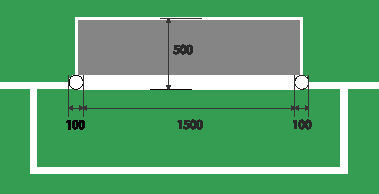
\includegraphics[width=1\columnwidth]{figs/goalDimensions2015.pdf}
\caption{Dimensions of the goal (in mm), viewed from above, and its placement on the field.}
\label{fig:goal_dimensions}
\end{center}
\end{figure}

\begin{figure}[h!]
\begin{center}
\leavevmode
\begin{minipage}[t]{0.49\columnwidth}
\imagebox{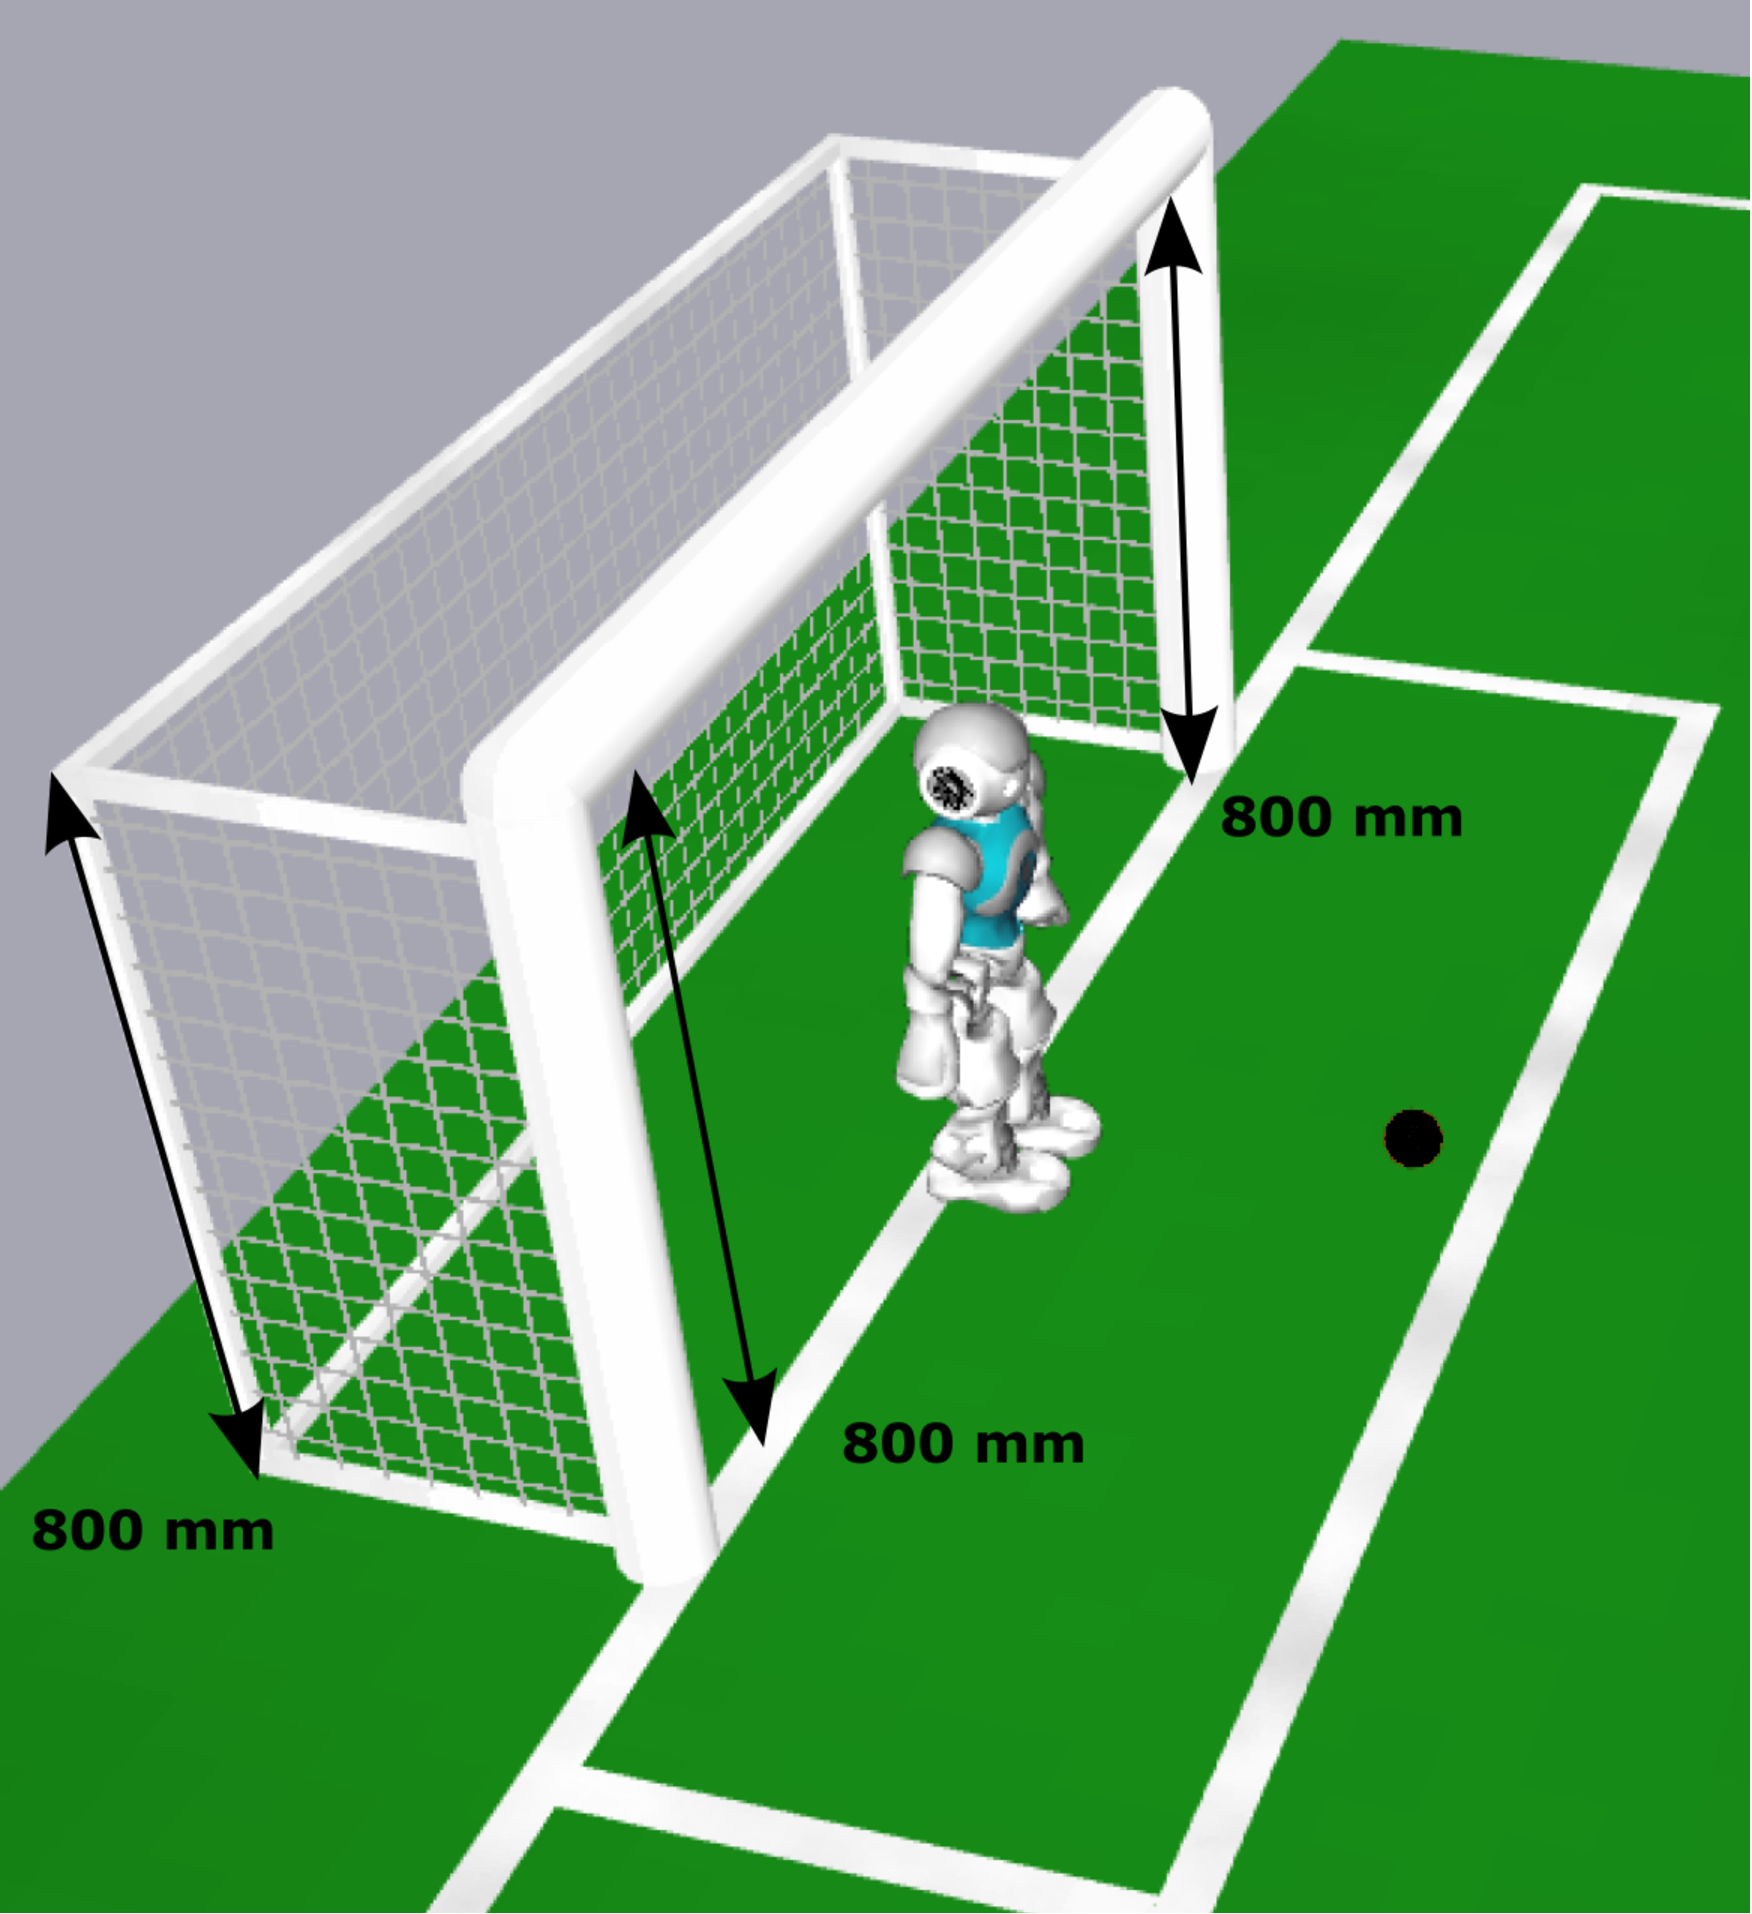
\includegraphics[width=1\columnwidth]{figs/goalDimensions3D.pdf}}%
\end{minipage}
\begin{minipage}[t]{0.49\columnwidth}
The goalposts and crossbar are made from 3 white cylinders with a diameter of \qty{100}{\milli\metre}.
The net:
\begin{itemize}
\item has a height of \qty{800}{\milli\metre}
\item is of white, gray or black color
\item is tightly supported via the support structure, in a way to minimize interference with the goalkeeper
\item has a weave with holes smaller than the ball diameter.
\end{itemize}
\end{minipage}
\caption{Appearance and dimensions of the goals.}
\label{fig:goal_appearance}
\end{center}
\end{figure}

\subsection{Field Colors}
\label{sec:field_colors}
The colors of the soccer field are as follows:

\begin{itemize}

\item The field (artificial turf) itself is green (color is not specified, but it should not be too dark).

\item The lines on the field are white, whether they are taped, spray painted or made from white artificial turf.

\item The posts and top crossbar of both goals are white. The net and the support structure for the net are white, gray, or black.

\end{itemize}

\subsection{Lighting Conditions}
\label{sec:lightConditions}
The lighting conditions depend on the actual venue. SPL fields should be placed near or under windows where possible. Whether window lighting is used, ceiling lights should be provided as necessary to ensure that most of the field is never darker than 300 Lux (400 Lux preferred).

Lighting is not required to be even and hotspots may occur on the field. The lighting design (comprising both natural and artificial light sources) shall aim to limit the ratio between the brightest and darkest patches on the field to less than 10:1. In general, lighting irregularities, including changes that occur during the competition, are acceptable and will not be cause for delay.  Such irregularities may include sun streaming through windows, light bulbs turning off, light bulbs being replaced, etc.

\subsection{Venue Setup}
\label{sec:boundaries}
Fields may be located close to one another.  Barriers will not necessarily be constructed between adjacent fields to block the robots from seeing other fields, goals, or balls. However, barriers will be constructed to block sight between any fields that are not located at least three meters apart. Hence, for each side of a field that is adjacent to another field, either barriers will separate the fields or at least \qty{3}{\metre} will be between the carpet of adjacent fields.

\subsection{Ball}
\label{sec:ball}

The official ball is a soft foam ball with a black and white soccer ball print (see \cref{fig:ball}). They are \qty{100}{\milli\metre} in diameter and weigh \qty{44}{\gram}. These balls are available by writing to \url{info@sportpaint.de} (in German or English) and asking to order the ``pu schaumstoffball 10cm 100ss''.  Each ball costs \euro{2.86} plus shipping, where shipping cost depends on the destination.

\begin{figure}[t]
  \centerline{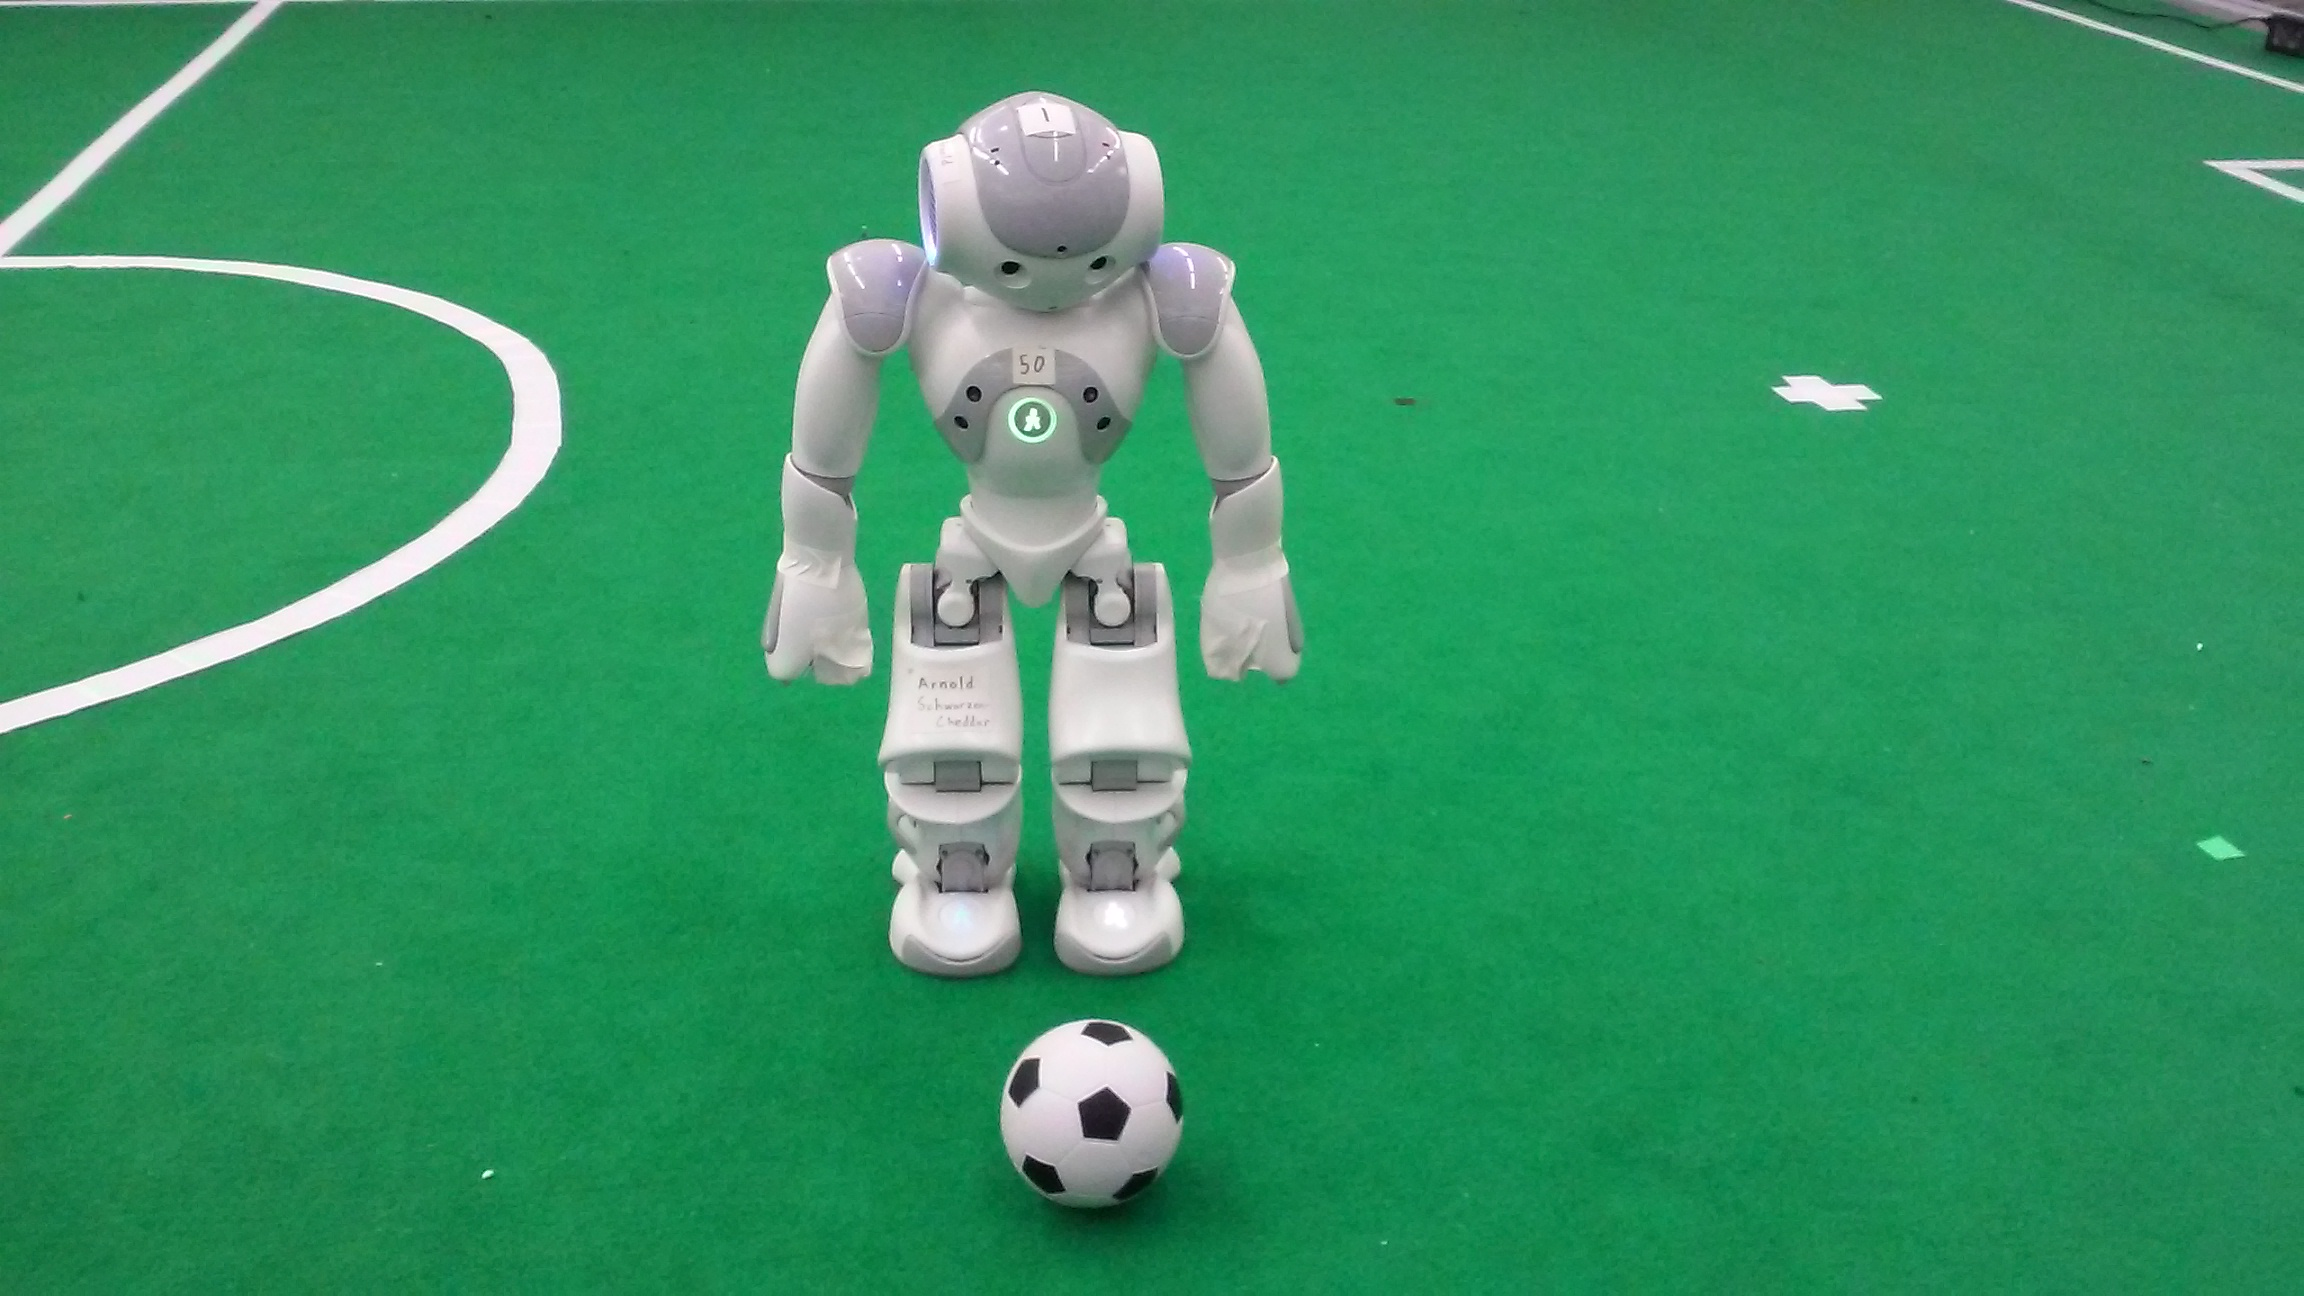
\includegraphics[height=0.28\columnwidth]{figs/robotWithBall2016.jpg}}
  \caption{A NAO and an official ball.}
  \label{fig:ball}
\end{figure}

\subsection{Definition of Inside and Outside}
\label{sec:inside_outside}

A line is always part of a region of the field.
This means, that \emph{inside/outside \textless region\textgreater} refers to the green area as well as the surrounding line.
Specifically:
\begin{itemize}
    \item The field boundary lines are part of the field
    \item The penalty area lines (and the adjacent part of the goal line) are part of the penalty area
    \item The center circle lines are part of the center circle
\end{itemize}

The only \textit{exception} to this rule is the halfway line, which does not form part of any half.
That is, a robot is \textit{outside} a half of the field if it is touching the halfway line.

\subsection{Streaming Setup}
\label{sec:streaming_setup}

There are multiple use cases for a streaming setup:
\begin{itemize}
    \item Stream all videos to RoboCup SPL Youtube channel to store them there
    \item Allow team members from remote to watch their robot's match
    \item Evaluate team's performance measures online from videos recording (Part of Technical Challenge 2022)
\end{itemize}

\newpage

% !TeX root = ../SPL-Rules.tex
% !TeX spellcheck = en_US
\section{Robot Players}
\label{sec:robot_players}
A match is played by two teams, each with a maximum of 5 or 7 players, depending on the competition rules.
At most one player per team on the field may be designated as \emph{goalkeeper}, the others are all \emph{field players}.
When playing at full strength, a team must have a \emph{goalkeeper} on the field.

In addition, each team may prepare \emph{substitute players} outside of the field. A \emph{substitute player} may be substituted in to become a \emph{field player} or \emph{goalkeeper}.

Each of the players has a unique jersey number from the set $\{1, 2, 3, \ldots, \MaxJerseyNumber\}$.

\subsection{Hardware}
\label{sec:hardware}
All teams must use black, gray, red, blue, or orange plated NAO humanoid robots manufactured by Aldebaran.

Absolutely no modifications or additions to the robot hardware are allowed. No additional hardware is permitted including off-board sensing or processing systems. Additional sensors besides those originally installed on the robots are likewise not allowed. The only exceptions are:

\begin{itemize}
    \item Setting the passive wrist joints to a fixed position either with glue or a transparent or white duct tape.
    \item Protecting the fingers with white finger protectors provided by the manufacturer or with transparent or white duct tape.
    \item Placing white duct tape over the battery case and screw (under the robot jersey) to keep the battery case in place and prevent the battery becoming disconnected.
    \item A memory stick may remain in the head during operation.  Only ordinary USB flash memory keys that sit flush or recessed to the head casing may be utilized. Other USB dongles or devices, as well as memory sticks that are not flush or recessed, are not permitted.
\end{itemize}

A computer with two monitors (one for GC and one for TCM) will be provided by the event organizers for the purpose of sending GameController messages to the robots and observing if no robot violates the rules for wireless network usage.
Additionally, there should be at least one monitor mirroring the second screen of the GC PC showing the GameState Visualizer.

\subsection{Team Markers}
\label{sec:team_markers}

Robots use colored jersey shirts as team markers. Each jersey shirt has a player number (1--\MaxJerseyNumber) printed on it.  The team markers are worn as shown in \cref{fig:nao_markers}.

\begin{figure}
  \centerline{\begin{tabular}{lll}
      a) & b) & c) \\
      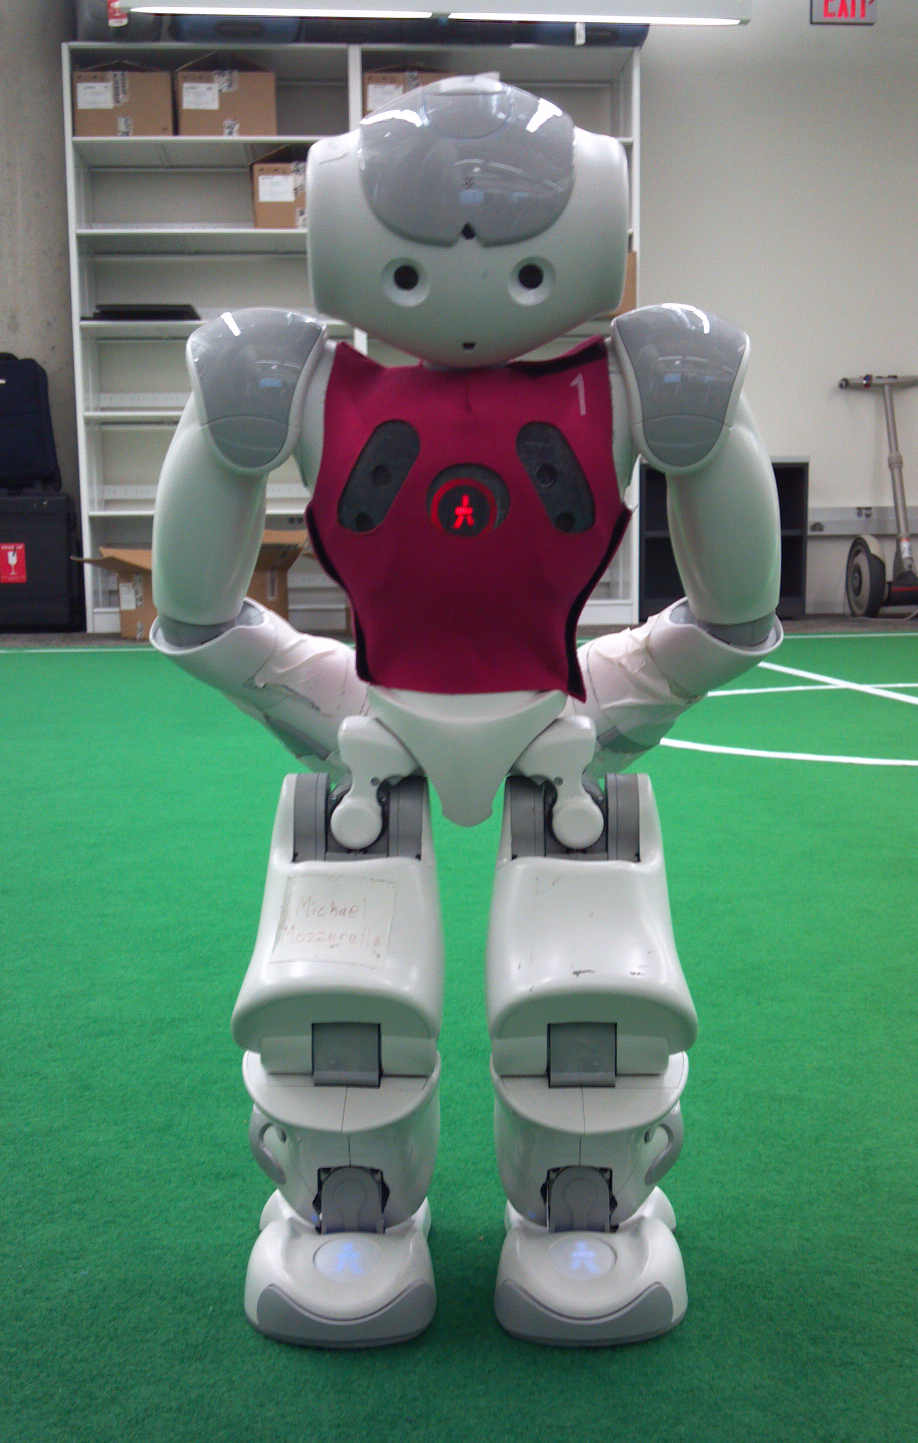
\includegraphics[height=0.28\columnwidth]{figs/front.jpg}&
      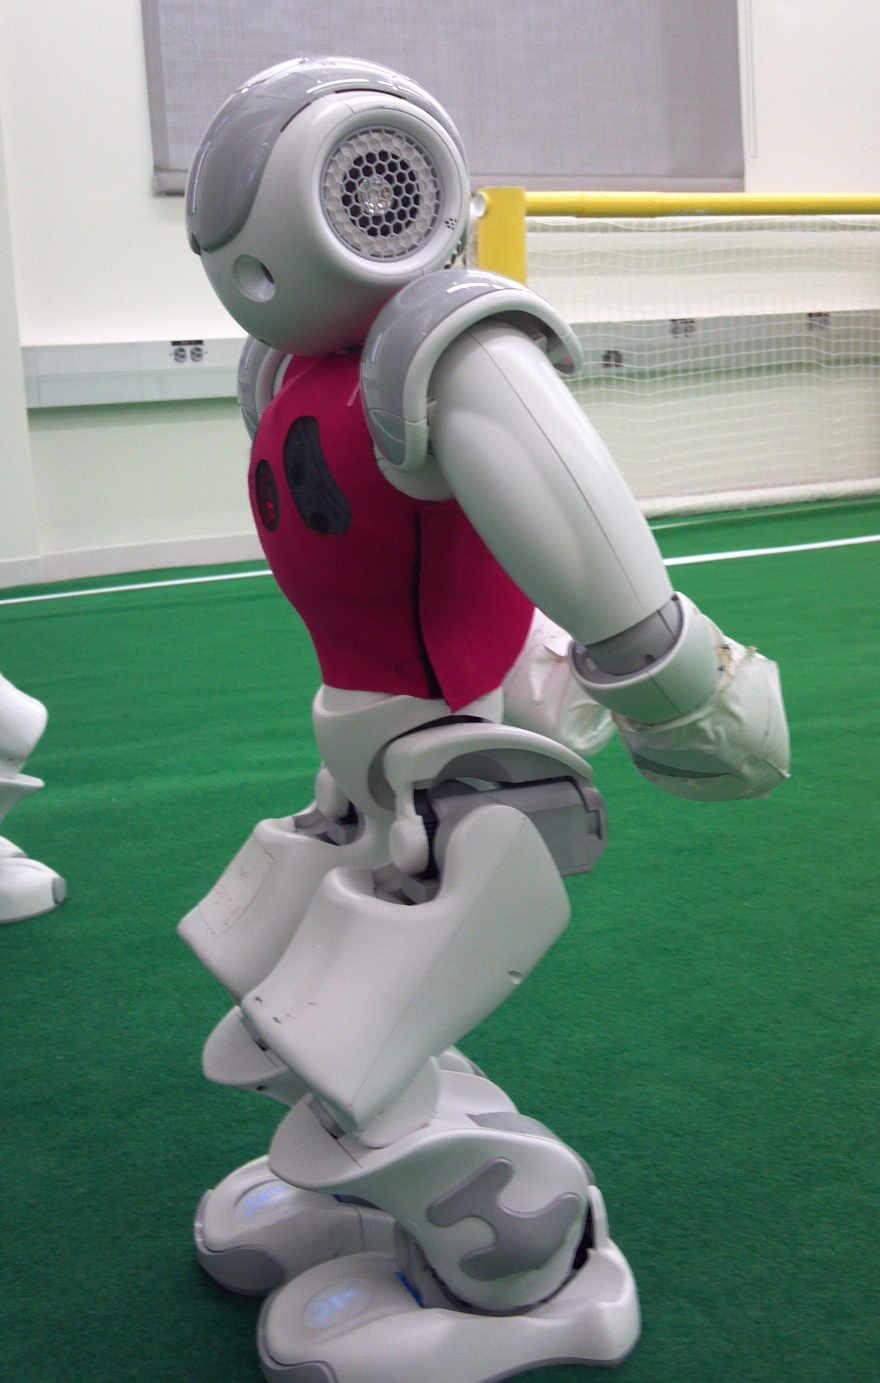
\includegraphics[height=0.28\columnwidth]{figs/side.jpg} &
      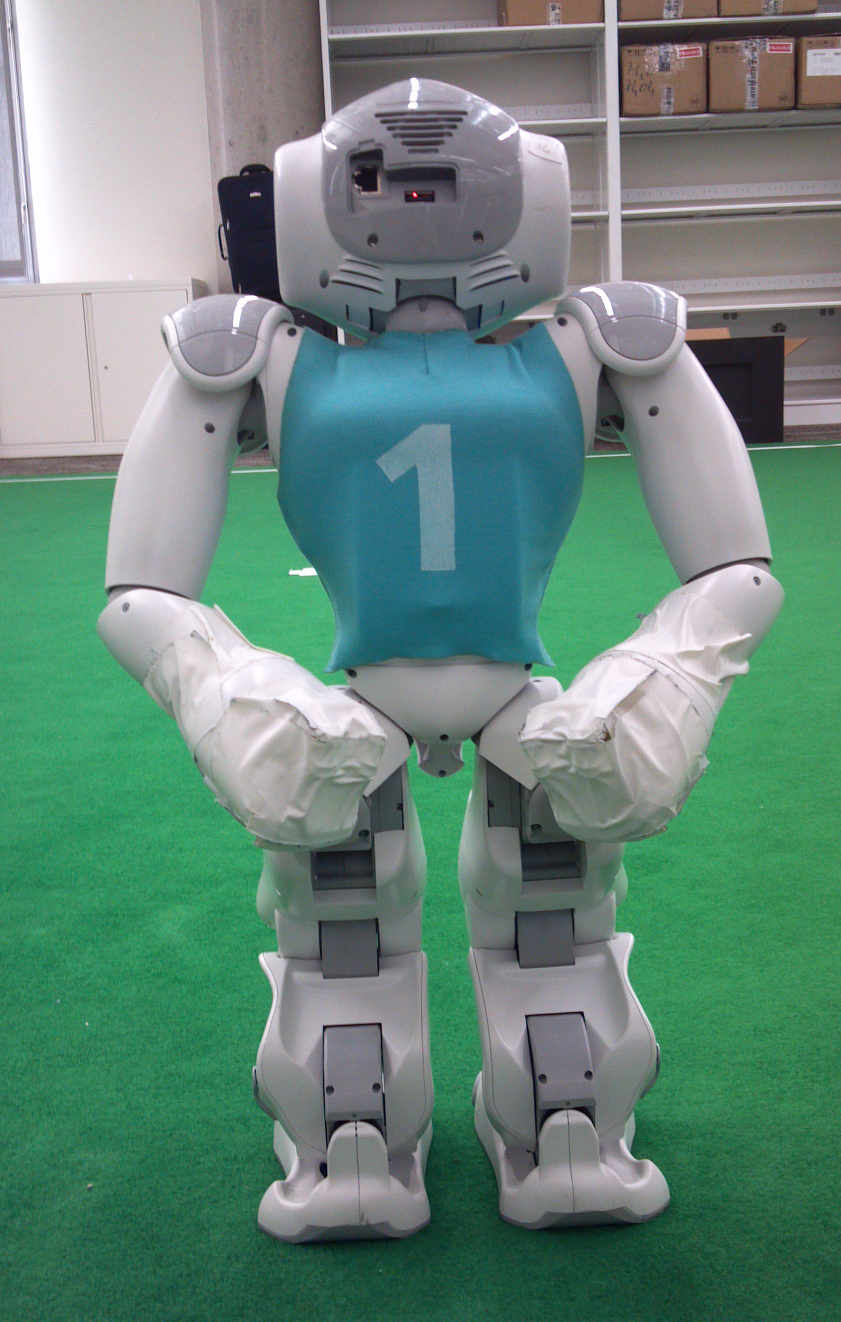
\includegraphics[height=0.28\columnwidth]{figs/back.jpg}
  \end{tabular} }
  \caption{Team markers. a) Front view. b) Side view. c) Back view.}
  \label{fig:nao_markers}
\end{figure}
Teams may use any jersey that was approved for a RoboCup SPL competition in the last 4 years without needing to approve it in \RCYear again.

Teams may design and manufacture their own jerseys in any color (multi and many color jerseys are acceptable), but must follow these guidelines:
\begin{itemize}
\item Jerseys should be the \textbf{tank top} style used at RoboCup 2013/2014 and should cover approximately the same areas of the robot as shown in \cref{fig:nao_markers}. The torso LED must be clearly visible. Jerseys may include the sonar panel used in the 2013/2014 jerseys, although this is not required. Jerseys may not cover the shoulders of the robots.
\item Jerseys must have a primary color that comprises more than half of the jersey.  The primary color must be recognizable from the front and back.
\item Jerseys should not contain distractors, such as large pictures of SPL balls or white stripes on green jerseys.
\item A team must wear the jerseys that it starts a game in for the entire game.
\item Jersey material must be non-reflecting and non-shiny.  Material that is glittery is also not appropriate.  Jerseys may be manufactured from fabric and fine mesh.
\item Jerseys should be numbered 1--{\MaxJerseyNumber} on both sides.  The numbers must be large and {\bf easily} recognized by humans.
\item Teams must have two sets of jerseys for \emph{field players} that are significantly different in terms of their primary color.
\item Teams must have two sets of jerseys for \emph{goalkeepers} that are significantly different in terms of their primary color.  One of the \emph{goalkeeper} primary colors must be different from both primary colors used for \emph{field players}.
\item Designs must be submitted to \url{rc-spl-tc@lists.robocup.org} for approval by \DTMdate{\JerseyApproveSubmissionDate}. If the team has jersey prototypes, they should submit close-up images of a robot wearing the jersey---these images should be taken from front, back, and side angles.  If the team has no prototypes, then designs depicting the expected jersey should be submitted.  If submissions show separated front and back halves of jerseys then the team must specify which halves are matched to form home and away jerseys.  All images and designs should be submitted in pdf or jpg format.
\end{itemize}

Each team must designate a ``home'' color and an ``away'' color for their \emph{field players} when asked about one month before RoboCup. Teams must wear their ``home'' jerseys when they are ``home'' (the first team listed on the schedule). Teams will wear their ``home'' jersey when they are ``away'' (the second team listed on the schedule) as well, unless either the head referee or the GameController program believes the jerseys of two competing teams are too similar.  In this case, the ``away'' team will then wear their ``away'' jersey.

Some teams wish to include additional information or logos on their robots. The following are allowable:

\begin{itemize}
  \item Adding sponsor or team logos to the upper legs of the robots (\cf \cref{fig:sponsor}). A box drawn around the non-white area of any logos must not cover more than a \qty{25}{\square\centi\metre} area.

  \item Adding small black and white stickers to the torso and/or head of the robots stating the name of the robot, the name of the team, or similar information. These stickers must be small and mostly white.
\end{itemize}

\begin{figure}
  \centerline{\begin{tabular}{ll}
  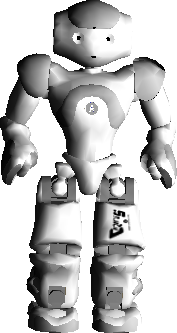
\includegraphics[height=0.35\columnwidth]{figs/naosim_with_logo.png}&
  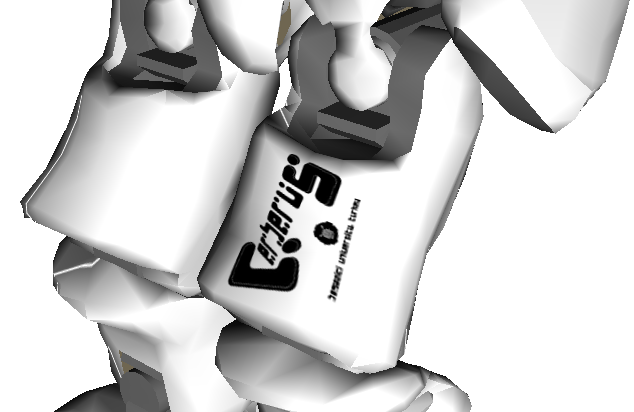
\includegraphics[height=0.35\columnwidth]{figs/naosim_legs_with_logo_closeup.png}
  \end{tabular}}
  \caption{Example Sponsor/Team Logo placement on legs.}
  \label{fig:sponsor}
\end{figure}

\subsection{Goalkeeper}
\label{sec:goalkeeper}

The \emph{goalkeeper} may use any of the allowed jersey numbers. The \emph{goalkeeper} must wear a jersey with a primary color different from the primary colors used by the \emph{field players} of both teams.

\subsection{Communications}

The robots must play without human control. Communication is only allowed among robots on the field and between the robots and the GameController.

\subsubsection{Non-wireless Communications}
\label{sec:acoustic}
In general there are no restrictions on communication between robots in play on the field using visual signalling (\eg gestures) or the robot's built-in microphones, speakers, and infrared transceivers. However, communication that causes excessive discomfort to an audience, affects the safety of an audience, or violates normal playing rules is not permitted.

\subsubsection{Wireless Communications}
\label{sec:wireless}
The only wireless hardware allowed to be used by the teams are the wireless network cards built into the NAOs, and the access points provided by the event organizers. All other wireless hardware must be deactivated. A team may be disqualified if one of the team members violates this rule.

Each team will get a range of IP addresses that can be used both for their robots and their computers. The network configuration (\eg IP addresses, channels, SSIDs, and required encryption) of the fields will be announced at the competition site.

Wireless robot-to-robot communication among the robot players is allowed, as long as it uses the access points provided by the event organizers (using the so-called ad-hoc mode is prohibited), messages are sent via UDP broadcast, and the SPL standard message format is used. The SPL standard message format is specified in the header \emph{SPLStandardMessage.h} that is distributed with the latest GameController release at \url{https://github.com/RoboCup-SPL/GameController}.

Each team will be assigned a range of IP-addresses that can be used for robot-to-robot communication. Each team will also be allocated a single UDP port for network broadcasts. Specifically, a team's port will be 10000 plus that team's GameController number. All robot-to-robot communication during matches must be sent via UDP broadcast. Unicast communication between robots is prohibited.

The amount of data transmitted by a team in a single game is limited. The limit is measured as the total number of UDP packets sent by any robots of a team. A team may not exceed \qty{\TeamMessageLimit}{packets} per game. For each minute of irregular extra time (\cf~\cref{sec:extra_time}), the limit is increased by \qty{\TeamMessageLimitMinute}{packets}. However, this does not apply to a team that has already exceeded its limit before. The GameController tracks the number of messages that have already been sent and includes counters for packets remaining per team in \texttt{RoboCupGameControlData}.

If a team exceeds their limit the game is scored with 0 goals for the offending team. Robot-to-robot communication that violates the SPL rules result in a game scored with 0 goals for the offending team (even when discovered after the game was finished). Messages are counted towards the limit during the \texttt{ready}, \texttt{set} and \texttt{playing} states. Limits do not apply during penalty kick shoot-out. If a knock-out game results in a draw and both teams exceeded their message limit, the team last exceeding their limit wins the game.

The limit of allowed packets will be lowered in future competitions to encourage smart event-based communication.

In addition to robot-to-robot communication, robots may send:
\begin{itemize}
 \item Additional status update packets that are sent to the GameController.
 \item Team specific debug information may be sent to an external computer owned by the team. A robot may send debug information at most once every \qty{2}{\second} in a single UDP packet.
\end{itemize}
These additional packets do not count towards the team's data limit and may not be used for robot-to-robot communication. They must be sent as unicast and may not be sent as broadcast.

Teams and their robots must not listen into another team's communication.

Robots are not allowed to be connected to access points of fields that are currently running official games of other teams.
Robots may only communicate on fields that are not running an official game or fields which they are playing on.

The GameController will use UDP to connect to the robots. The source distribution of the GameController provides the header file \emph{RoboCupGameControlData.h} that defines all messages sent by the GameController to the robots. They correspond to the \emph{robot states} described in \cref{sec:robot_states}.

Robots send status updates (defined in \emph{RoboCupGameControlData.h}) to the GameController. These return packets must be addressed directly to the GameController PC (\ie not broadcast) and sent on the GameController return UDP port specified by the symbol \verb!GAMECONTROLLER_RETURN_PORT! in \emph{RoboCupGameControlData.h}.

The use of remote processing/sensing is prohibited.

\newpage

% !TeX root = ../SPL-Rules.tex
% !TeX spellcheck = en_US
\section{Game Process}
\label{sec:game_process}

\subsection{Structure of the Game}
\label{sec:game_struct}

A game consists of four parts, pre-game meeting (see~\cref{sec:referee_team_communication}), the first half, a half-time break, and the second half.
Each half is \qty{10}{\minute} counted from the initial kick-off.
The half-time break is \qty{10}{\minute}, and during this time both teams may change robots, change programs, or do anything else that can be done within the time allotted.

The head referee signals the commencement of each half with a single whistle blow (that is, the Initial kick-off, \cf \cref{sec:initial-kick-off}).
The head referee signals the end of the first half with two short whistle blows, and the end of the second half with two short plus one long whistle blow.
The head referee should make \textit{all} of these whistle sounds from the T-junction of the halfway line.

\subsection{Robot States}
\label{sec:robot_states}

Robots can be in \textit{eight} different \emph{primary} states (see~\cref{fig:robot_states}).
Wireless connection must be available, so these states will be set by the GameController.
Teams must implement code to receive and correctly respond to wireless GameController packets, and also give a visual indication of the game state.

\textbf{The usage of the button interface as a replacement for any GameController commands/transitions is not allowed in the main competition!}

Should, on both teams, at least two robots have problems with the wireless network or GameController connection the head referee should issue a referee timeout (see \cref{sec:referee_timeout}).
If fewer robots do not respond to the GameController then they are, at the beginning, not included in the game (via a `Request for Pick-up', see \cref{sec:request_for_pickup}), and the game starts without the offending robot.

The primary states are:
\begin{description}
  \item[Unstiff.] It helps to facilitate a consistent and safe handling of the robots for remote competition.
    During any state, if all head buttons are pressed at least one second, the robot should move to a safe seated/crouched position and unstiffen all joints.
    So while in the \texttt{unstiff} state the robot is not allowed to move in any fashion! After booting, the robots are in their \texttt{unstiff} state.
    Pressing the chest button once while in the \texttt{unstiff} state, permits the robot to stiffen its joints and return to the \texttt{initial} state, or a state as indicated by GameController.

  \item[Initial.] The robots are not allowed to be moving in any fashion besides initially standing up.
    Shortly pressing the chest button will switch the robot to the \texttt{penalized} state.

  \item[Ready.] In this state, the robots walk to their legal positions for kick-off (\cf \cref{sec:kick-off}) or a penalty kick (\cf \cref{sec:penalty_kick}).
    They remain in this state, until the head referee decides that there is no significant progress, up to a maximum of \qty{\KickOffAutoTime}{\second} for a kick-off and \qty{\PenaltyKickSetupTime}{\second} for a penalty kick.
    The GameController can activate sub-states for kick-off and penalty kicks.

  \item[Set.] In this state, the robots stop and wait for kick-off (\cf \cref{sec:kick-off}) or a penalty kick (\cf \cref{sec:penalty_kick}).
    Illegally positioned robots are \texttt{penalized} and placed on the side of the field.
    Robots are allowed to move their heads and arms or get up if fallen before the game (re)starts, but they are not otherwise allowed to move their legs or locomote in any fashion.
    If a robot cannot get up, fallen robot is called~(\cf \cref{sec:fallenrobots}).
    The penalty time counter is frozen during this state.
    Note that all penalized robots are left in place (on the side of the field, or in-place for motion in set) and must wait to get unpenalized.
    The GameController can activate sub-states for kick-off and penalty kicks.

  \item[Playing.] In the \texttt{playing} state, the robots are playing soccer.
    Shortly pressing the chest button will switch the robot to the \texttt{penalized} state.
    During the \texttt{playing} state, the GameController can activate the sub-states for free kicks (\cf \cref{sec:free_kick}).

  \item[Penalized.] A robot is in this state when it has been \texttt{penalized}.
    The only allowed movement is standing up after falling.
    Any other movement (including turning the head) is disallowed.
    Shortly pressing the chest button will switch the robot back to the \texttt{playing} state.

  \item[Finished.] This state is reached when a half is finished.

  \item[Calibration.] This state denotes the robot is acting with automatic calibration.
    This state may only be entered from \texttt{initial} by first pressing the front head button concluded by the chest button, for at least one second by the referees.
\end{description}

\begin{figure}[t]
  \centerline{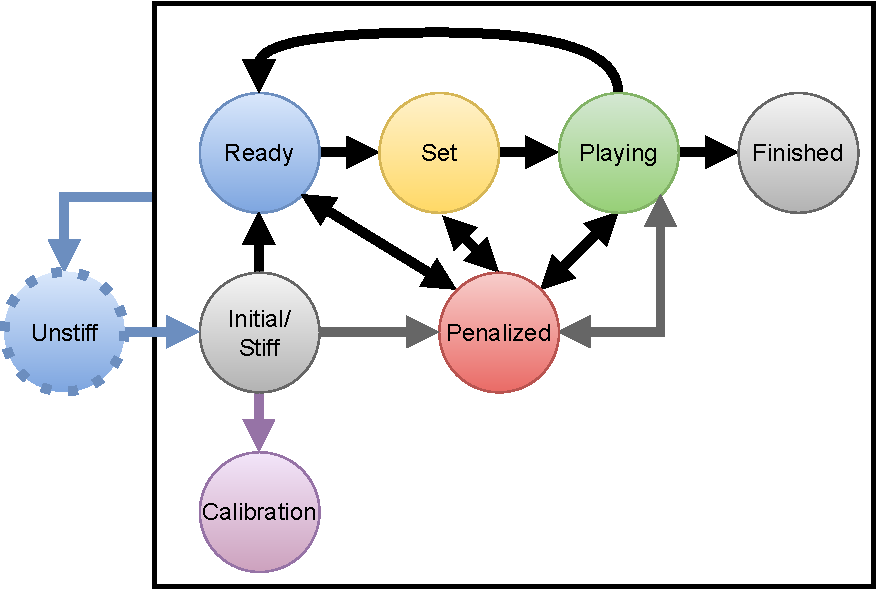
\includegraphics[width=0.9\columnwidth]{figs/states_new.pdf}}
  \caption{Diagram of the robot states.
    \\\textbf{Chest button} transitions are shown as gray arrows.
    However, any transition possible should be sent by the GameController.
    \\\textbf{GameController} transitions are shown as black arrows.
    \\Calibration transitions are shown as purple arrows which mean pressing the \textbf{front head button + the chest button}.
    \\From any state it can be transitioned to the \texttt{unstiff} state, shown as a blue arrow, via pressing all \textbf{three head buttons}.
    Pressing the \textbf{chest button} in the \texttt{unstiff} state allows a transition to the \texttt{initial} state, or a state as indicated by the GameController.}
  \label{fig:robot_states}
\end{figure}

The referee will announce the start of the \texttt{ready} state for both halves by raising both hands covered with red gloves \footnote{Teams are encouraged to not rely on the red gloves as they could be removed in the a following years.}.
The GameController \texttt{ready} signal will be delayed by \qty{\SetDelayTimeChampion}{\second} for champion cup and by \qty{\SetDelayTimeChallenger}{\second} for challenger shield. 
The referee must stand on the side of the field at halfway line level. 

The referee will announce the start of the \texttt{playing} state with a single whistle blow.
The GameController \texttt{playing} signal will be delayed by \qty{\PlayingDelayTime}{\second}.
This delay applies to both kick-off and penalty kicks.

The current game state should be displayed on the LED in the torso.
The colors corresponding to the game states are:
\begin{itemize}
  \item \texttt{Unstiff}: Blue-Blinking
  \item \texttt{Initial}: Off
  \item \texttt{Ready}: Blue
  \item \texttt{Set}: Yellow
  \item \texttt{Playing}: Green
  \item \texttt{Penalized}: Red
  \item \texttt{Finished}: Off
  \item \texttt{Calibration}: Purple
\end{itemize}

The current GameController requires robots to know both their team number and their robot number within the team.
It is each team's responsibility to make sure this is correctly configured.
It is recommended that the robot indicates its number within the team on boot up so that this can be easily checked at the start of the game.

\subsection{Goal}
\label{sec:goal}

A goal, including own goal, is achieved when the entire ball (not only the center of the ball) goes over the goal-side edge of the goal line, \ie the ball is completely inside the goal.\footnote{
  The goal line is part of the field.
}

The head referee signals a goal by a single whistle blow, followed by the call ``Goal \textless color\textgreater''.
The head referee should point with one arm towards the center of the field.
To assist robots listening for whistles, the referee should blow the whistle from on the carpet at the end of the fields where the goal was scored.

After a team scores a goal, the game proceeds with a kick-off (\cf~\cref{sec:kick-off}) for their opponents.
The GameController signal (to the robots) of a goal being scored, will be delayed by \qty{\GoalScoredDelay}{\second}.

\subsubsection{Invalid Goal}
\label{sec:invalid_goal}

A goal is invalid (that is, it can never be awarded) in the following circumstances:
\begin{enumerate}
    \item When an indirect kick is required but has not occurred (see~\cref{sec:indirect_kick}).
    \item When the last contact of the ball was with an attacking robot that played the ball with the arms/hands as defined in \cref{sec:hand_ball}.
      However, an own goal may be scored by any defending robot playing with arms/hands.
    \item When a team scores on themselves and there are no opponent robots on the field that are active (a definition of \emph{active} is given in \cref{sec:fallenrobots}).
\end{enumerate}

In these cases a goal is not scored (that is, the goal is ruled invalid), and the game will proceed with a Goal Kick (\cf \cref{sec:free_kick}).
The head referee should also advise why the goal is invalid, such as by calling ``Not indirect'', ``Played with hands'' or ``No own goal''.

\subsubsection{Indirect Kick}
\label{sec:indirect_kick}

The attacking team may only score a goal via indirect kick from any restart into \texttt{playing} from a free kick.

\begin{itemize}
  \item A robot may not score a goal from a direct kick, including via deflections.
  \item The ball must be deliberately played-at a second time (by either another robot, or the same robot) before a goal may be scored.
    A deliberate play at the ball includes successfully kicking the ball, dribbling the ball (and subsequently leaving possession of the ball), or the goalkeeper playing at the ball with its hands.
  \item If a robot plays the ball to itself, this means that the ball must leave a circular area of at least \qty{0.75}{\metre} around the robot before the ball is played a second time and to be considered as an indirect kick.
  \item Note that an own-goal may always be scored without requiring an indirect kick.
\end{itemize}

\begin{description}
  \item[Example 1:] Player 2 (of the red team) kicks the ball to Player~3, who then kicks the ball into the blue-team's goal.
    This is a successful indirect kick, and the goal counts.
  \item[Example 2:] Player 2 (of the red team) kicks the ball at the goal, and it is deflected of the side of the foot of a blue-team's robot into the goal.
    This is \textit{not} an indirect kick, and the goal does not count.
  \item[Example 3:] Player 2 (of the red team) kicks the ball ``upfield''.
    A blue-team robot kicks the ball a short distance, after which Player~2 kicks the ball again into the blue team's goal.
    This is a successful indirect kick, and the goal counts.
  \item[Example 4:] Player 2 (of the red team), walks up to and dribbles the ball.
    To be an indirect kick, Player~2 must then stop, and visibly back away from the ball, before approaching to dribble a \textit{second} time.
    The robot then scores.
    This is a successful indirect kick.
\end{description}

\subsection{Field-Side Selection and Initial Kick-off}
\label{sec:field_side_and_initial_kickoff}

\begin{itemize}
  \item The head referee throws a coin with one side for the home team and the other side for the away team according to the schedule.
    The team that wins the coin toss can either choose which goal to play for in the first half or take the kick-off.
  \item Depending on the decision above, the opposing team is given either the kick-off or may choose which goal to play for in the first half.
  \item The team that decided which goal to play for in the first half takes the kick-off at the start of the second half.
  \item In the half-time break both teams switch the sides of the field at play for the other goal.
  \item Teams must not change primary jersey colors for field players or goalkeepers during a match.
\end{itemize}

\subsection{Initial Kick-off}
\label{sec:initial-kick-off}

The first kick-off at the start of each half or after a timeout is an initial kick-off.
Robots have to be ready next to the field at latest \qty{2}{\min} before an initial kick-off.
All robots must be in the \texttt{unstiff} state.

Latest \qty{1}{\min} before the game starts all robots must be placed on the touchlines facing the other touchline in their own half by their team.
% (if present in person at the competition site) or their responsible referee according to \cref{fig:initial_positions}.
% If a team places robots themselves for initial kick-off, it is allowed for the team to vary the spacing and orientation of the robot positions along legal positions on their half's touchlines~(see also~\cref{sec:inside_outside}).

Robots are brought into the \texttt{initial} state after they are placed.
Once the robots receive the \texttt{ready} signal from the GameController, they proceed as described in \cref{sec:kick-off}.

% \begin{figure}[t!]
%   \begin{center}
%     \leavevmode
%     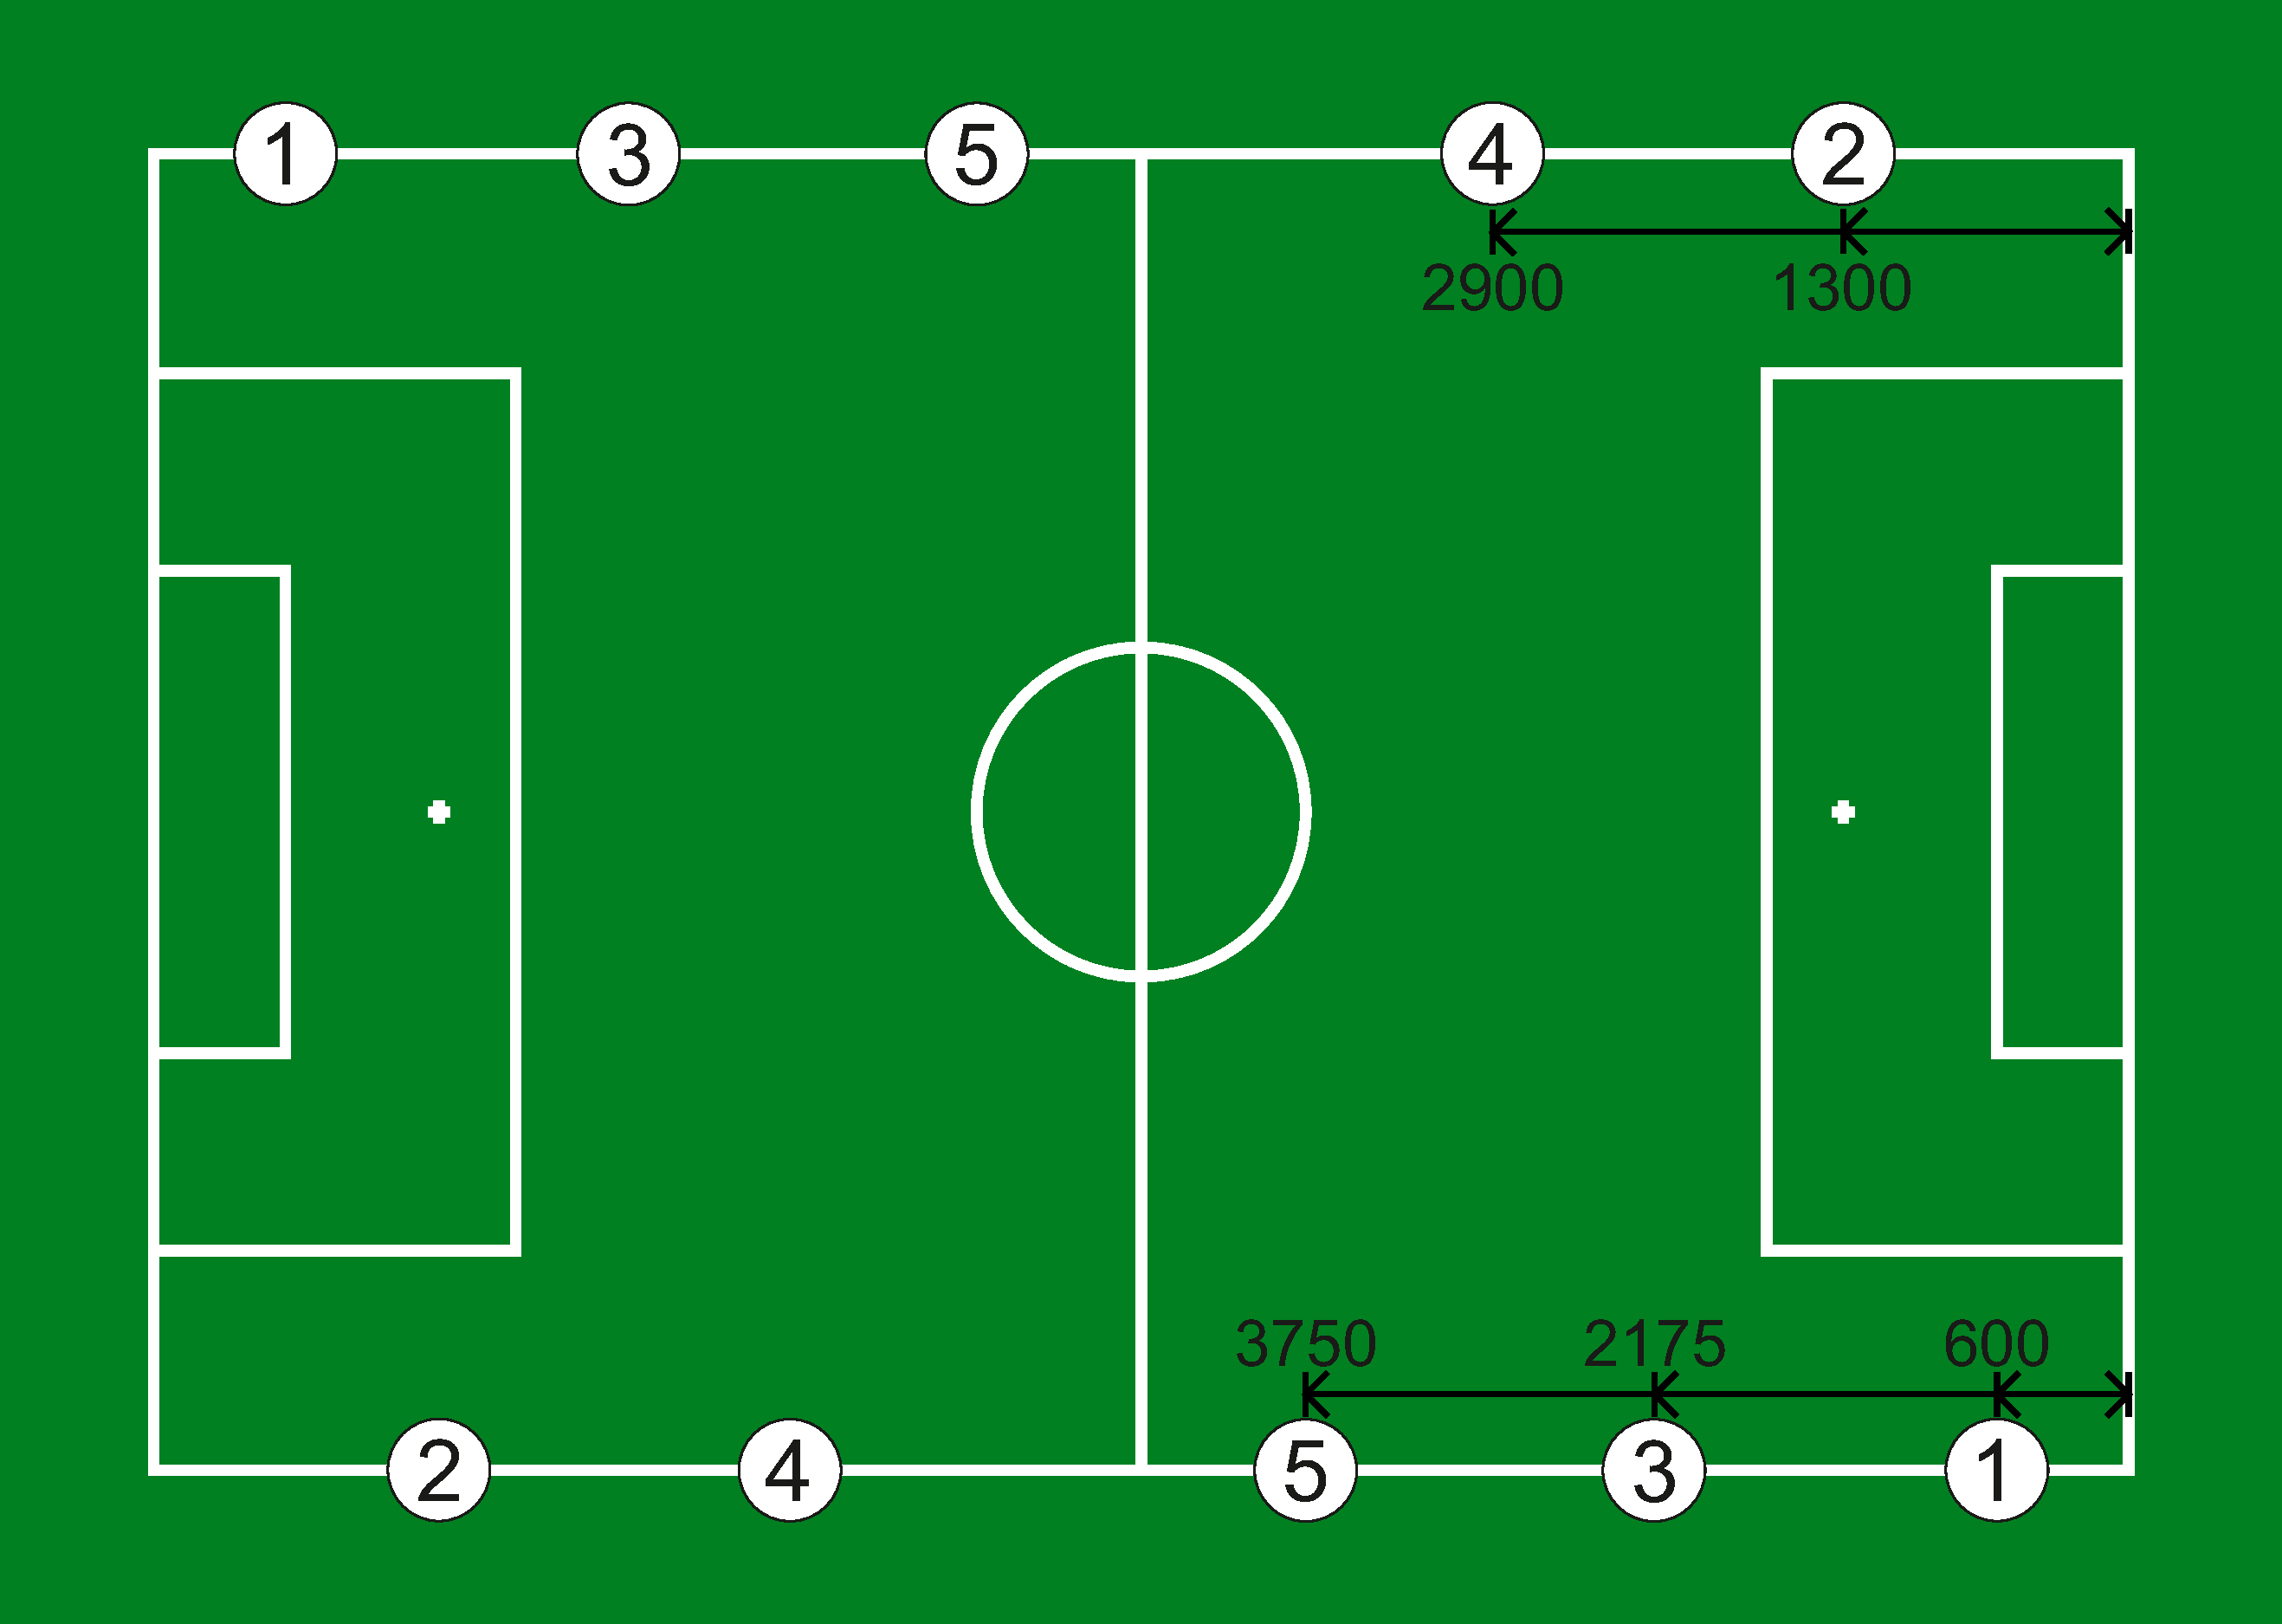
\includegraphics[width=1\columnwidth]{figs/initial_positions.pdf}
%     \caption{Positions, player numbers and distances from the center of the goal line for the initial kick-off of the robots.}
%     \label{fig:initial_positions}
%   \end{center}
% \end{figure}

\subsection{Kick-off}
\label{sec:kick-off}

For kick-off, the robots run through three states: \texttt{ready}, \texttt{set}, and \texttt{playing}.

In the \texttt{ready} state, the robots must walk to legal kick-off positions for their team.
Upon reaching the \texttt{set} state, the robots must stop and remain stationary until the kick-off is signaled by the referee (\cf~\cref{sec:motion_in_set}).
The following restrictions apply from the beginning of the \texttt{set} state until the ball comes into play:
\begin{itemize}
  \item The kick-off team can be positioned within their own half and the center circle.
    No robot may block the center mark.
    Up to one robot of the kick-off team is allowed to be outside the own half, provided it is inside the center circle.
    If more than one robot is outside the own half, only the one closest to the center mark is legal.
    This robot is then called \emph{kick-off} player and must execute the kick-off.
    If any other robot of the kick-off team executes the kick-off, the robot wrongly taking the kick-off is considered to be illegally positioned and a moved ball is placed back.
  \item The defending team can be positioned within their own half excluding the center circle.
  \item Robots are allowed to be positioned inside their own goal.
    All other positions that are fully on the border strip are illegal for both teams.
  \item Both teams are also subject to restrictions on the goal area (\cf~\cref{sec:ip_own_goal_area}).
\end{itemize}
All robots that do not reach legal positions before the \texttt{set} state begins or enter illegal positions before the ball is in play will be penalized with the ``Illegal Position'' penalty~(\cf \cref{sec:ip_kick_off}).

A referee places the ball on the center mark.
If the ball is moved by one of the robots during the \texttt{set} state, it is placed back by one of the referees.

The head referee signals the kick-off by a single whistle blow, followed by the call ``Playing''.
The head referee must signal this from the T-junction of the halfway line.
\qty{\PlayingDelayTime}{\second} after the head referee has signaled the kick-off, the robots' state is switched to \texttt{playing} by the GameController (regardless of when the ball comes into play).

A goal may be scored directly from a kick-off.

\subsubsection{Ball in Play}

The ball is in play and kick-off ends once
\begin{itemize}
  \item it is touched by the attacking team and moved clearly or
  \item \qty{\KickOffBallFreeTime}{\second} have elapsed in the \texttt{playing} state.
\end{itemize}

The GameController and head referee will indicate this by the call ``Ball Free''.

\subsection{Kick-in}
\label{sec:kick_in}

A ball is considered to have left the field when there is no part of the ball over the outside of the boundary line (\ie the line itself is in).
If the ball leaves the field it will be replaced on the field by an assistant referee.
Balls are deemed to be out based on the team that last touched the ball, irrespective of who actually kicked the ball.

If the ball goes over a touchline then the assistant referee will replace the ball back on the point of that touchline where it went out.
A free kick (\cf \cref{sec:free_kick}) is awarded to the team that did \emph{not} last touch the ball by the referee calling ``Kick-in \textless color\textgreater''.

If the ball goes over a goal line then the assistant referee will replace the ball back on the field, depending on which team last touched the ball.

\begin{itemize}
  \item If the ball was last touched by the defensive team, a \emph{Corner Kick} (\cf \cref{sec:free_kick}) is awarded to the attacking team.
    The referee calls ``Corner Kick \textless color\textgreater'' and the ball is placed on the corner on the same side of the field that the ball was kicked-out.
  \item If the ball was last touched by the offensive team, a \emph{Goal Kick} (\cf \cref{sec:free_kick}) is awarded to the defensive team.
    The referee calls ``Goal Kick \textless color\textgreater'', and the ball is placed on the corner of the goal area on the same side of the field that the ball was kicked-out.
    That is, the corner inside the field, not the T-junction where the goal area meets the goal line.
\end{itemize}

In these examples, ``red half of the field'' refers to the half the red team is defending.

\textbf{Example 1:} The red goalkeeper kicks the ball out the end of the field to the right of the goal.
The referee calls ``Corner Kick blue'', the ball is placed on the corner to the right of the goal and a free kick is started.

\textbf{Example 2:} A blue robot kicks the ball out the end of the field to the right of the goal the red team is defending.
The referee calls ``Goal Kick red'' and the ball is placed on the right corner of the goal area.

\textbf{Example 3:} A blue robot at midfield kicks the ball over the left touchline \qty{2}{\metre} into the red half of the field.
The referee calls ``Kick-in red'' and the ball is replaced on the left touchline where it went out.

\textbf{Example 4:} A blue robot kicks the ball but the ball touches a red robot at midfield before leaving the field near the halfway line.
The ball is regarded as out by red, the referee calls ``Kick-in blue'' and the ball is replaced on the touchline where it went out.

\subsection{Free Kick}
\label{sec:free_kick}

A free kick is initiated:
\begin{itemize}
  \item When the ball goes over the touchlines, termed \emph{Kick-in}.
  \item When the ball goes over the goal lines initiated by the defensive team, termed \emph{Corner Kick}.
  \item In place of a goal line Kick-in initiated by the offensive team, also termed a \emph{Goal Kick}.
  \item When a pushing penalty (see \cref{sec:player_pushing}) is awarded near the ball, termed a \emph{Pushing Free Kick}.
\end{itemize}

The head referee will announce a free kick, calling one of:
\begin{enumerate}
  \item For a \textit{Kick-in/Goal Kick/Corner Kick}: ``Kick-in/Goal Kick/Corner Kick \textless team\textgreater'' for the team that did not last touch the ball.
  \item For a \textit{Pushing free kick}: ``Foul \textless offending color\textgreater \textless offending number\textgreater'' for the pushing robot.
\end{enumerate}

The GameController will then activate the sub-state for the respective free kick.
Note that in the case of the Pushing free kick the sub-state is activated automatically through the ``Foul''.
The team who is awarded the free kick (termed the attacking team) has \qty{\FreeKickTime}{\second} to complete the kick.

When necessary, the referee may need to place the ball.
For a pushing free kick, the ball will be left in place, and only repositioned in accordance with the pushing rules (see \cref{sec:player_pushing}).
If the ball left the field, the ball will be positioned as described in \cref{sec:kick_in}.

During the free kick, only the attacking team may approach within \qty{\FreeKickRadius}{\metre} to the ball.
All robots of the defensive team must immediately move away from the ball.
Defensive robots that violate these restrictions are penalized with the ``Illegal Positioning'' penalty (see \cref{sec:illegal_positioning}) which results in a standard removal penalty~(see \cref{sec:removal_penalty}).
Additional penalties against any further robots during the free kick, including Pushing, do not result in an additional free kick, but still use the appropriate removal penalty.

A free kick is deemed completed and play returns to normal if:
\begin{itemize}
  \item The attacking team moves the ball clearly, except for a robot getting up which is exempt from this rule.
  \item The \qty{\FreeKickTime}{\second} time period expires (or the game time expires).
\end{itemize}
The head referee will announce a free kick is completed by calling ``Ball Free'', and the GameController resumes the game state \texttt{playing}.
Note that the sub-state will be automatically left after the \qty{\FreeKickTime}{\second} time period expires.

\subsection{Penalty Kick}
\label{sec:penalty_kick}

A penalty kick is initiated when a pushing penalty (see \cref{sec:player_pushing}) is awarded near the ball against the defending team within their own penalty area.
The head referee will announce a penalty kick by calling ``Penalty Kick \textless offending color\textgreater \textless offending number\textgreater'' for the pushing robot.

When the GameController activates the penalty kick, the game changes to the \texttt{ready} state with \texttt{penalty kick} sub-state active.

This denotes that the robots are given time to set up and prepare for the penalty kick.
Similar to kick-off, the game clock is \textit{paused} during finals games only.
The referees should pick up the ball.

Robots have \qty{\PenaltyKickSetupTime}{\second} to get into position for the penalty kick.
At the end of \qty{\PenaltyKickSetupTime}{\second}, the game changes to the \texttt{set} state with \texttt{penalty kick} sub-state active.
Similar to a kick-off, during the \texttt{set} state the robots are waiting for the penalty kick to commence.
Standard penalties apply.
Additionally, only the goalkeeper robot from the defending team may be within the penalty area.
The goalkeeper robot must either be touching the goal line or stay outside its own penalty area.
If the goalkeeper positioned itself inside the goal area but ahead of the goal line it is placed back by the referee during \texttt{set} state, so the center of its feet touches the center of the goal line.
The placement should happen perpendicular to the goal line without rotating the robot.
If this manual placement would lead to a position the robot collides with a goalpost, it is placed inside or outside the goalpost on the goal line, depending on which position is closer.
Only one robot from the attacking team may be within the penalty area, and it may not block the penalty mark.
Blocking the penalty mark is considered to be an illegal position.
All robots that do not reach legal positions will be penalized with the ``Illegal Positioning'' penalty~(\cf \cref{sec:illegal_positioning}).

The referee should also place the ball on the penalty mark during \texttt{set}.
The referee signals the penalty kick commences by blowing the whistle once, and calling ``Playing''.
The game switches to the \texttt{penalty kick} sub-state of the \texttt{playing} game state, and the game clock is resumed.
(Note that the GameContoller signal is delayed by \qty{\PlayingDelayTime}{\second} when switching from \texttt{set} to \texttt{penalty kick} sub-state).
The attacking team has \qty{\PenaltyKickTime}{\second} to complete the penalty kick.

During the penalty kick:
\begin{enumerate}
  \item The defensive goalkeeper robot must always be in contact with the goal line if it is inside the penalty area, and must remain on its feet.
    The goalkeeper is only permitted to ``dive'', and be off its feet after the attacking robot has touched the ball.
  \item The attacking robot may move freely.
  \item All robots must be within the field-of-play.
    That is, robots may not be outside the field lines, but within the field border.
  \item No other robots may enter the penalty area (\cf \cref{sec:illegal_positioning}).
  \item Additional penalties against any further robots, including pushing, do not result in an additional free
    kick, but still use the appropriate removal penalty.
\end{enumerate}

The attacking robot (taking the penalty kick) may only score a goal if it touches the ball once.
Once the attacking robot has touched the ball, it may not score a goal until another robot (from either team) touches the ball.
If this robot ``scores'', it results in a goal kick~(\cf \cref{sec:invalid_goal}).

The penalty kick is deemed completed if:
\begin{itemize}
  \item The attacking team touches the ball, even if the robot has fallen.
  \item The \qty{\PenaltyKickTime}{\second} time period expires (or the game time expires).
\end{itemize}

The head referee will announce a penalty kick is completed by calling ``Ball Free'', and the GameController resumes the game state \texttt{playing}.
Note that the sub-state will be automatically left (returning to the \texttt{playing} state) after the \qty{\PenaltyKickTime}{\second} time period expires.

Note that the restrictions on the attacking robot still apply after the penalty kick is complete.

\subsection{Game Stuck}
\label{sec:game_stuck}

In the event of no substantial change in the game state for \qty{\GameStuckTime}{\second}, this is considered a game stuck.
``Substantial change'' can consist of a robot seeing and moving towards the ball OR robots exploring the field (presumably in an attempt to find the ball).

The main referee has two options how to solve the game stuck and to reestablish the chance of progress in the game.
The intention of the game stuck rule is to achieve progress with as little intervention as possible, \ie the \emph{Local Game Stuck} rule will be preferred, but only if there is a chance that its application will result in progress in the game.

\subsubsection{Local Game Stuck}
\label{sec:game_stuck:local}

If one robot is preventing the game from proceeding---perhaps by circling the ball repeatedly without kicking the ball---it is recommended to improve progress by removing this one robot.
The head referee calls ``Local Game Stuck \textless robot\textgreater'' for this robot, which is penalized (\cf \cref{sec:pen_local_game_stuck}).

\subsubsection{Global Game Stuck}
\label{sec:game_stuck:global}

If no robots have made progress towards the ball or began to explore the field in \qty{\GameStuckTime}{\second} Global Game Stuck should be called on the team whose robot is \textit{not} nearest the ball.
The referee calls ``Global Game Stuck \textless color\textgreater''.

Once the referee calls Global Game Stuck, players enter the \texttt{ready} state, and a new kick-off is awarded to the team that was closer to the ball when the Global Game Stuck was called.
A global game stuck can only be called if at least one robot has touched the ball since the previous kick-off.

\subsection{Request for Pick-up}
\label{sec:request_for_pickup}

Either team may request that one of their players be picked up (called ``Request for Pick-up'').
In the \texttt{playing} or \texttt{ready} state, players may only be picked up for hardware failures.
In all other states, players may be picked up for any reason.

Every change (hardware or software) is allowed during a request for pick-up.
In particular, it is permitted to change batteries, fix mechanical problems, reboot the robots, and change configuration files.
It is also allowed to replace a broken robot by a substitute robot.
Substitute robots must wear the correct jersey color for their role (goalkeeper or field player).
It is discouraged to change the robot's control program, \textbf{but not forbidden}.

Any strategic ``Request for Pick-up'' is not allowed.
That is, gaining an advantage by removing the robot from the game.
In this case, the head referee will indicate when the robot is no longer affecting play and can be removed from the field by an assistant referee.

To prevent mistakes and confusion during games, only team captains (\cf \cref{sec:referee_team_communication}) should make a ``Request for Pick-up'', and only one designated person per team shall accept the robot from the referee, and hand it back after fixing the problem.
The returning robot may be returned following the normal replacement procedure once at least \qty{\StandardPenaltyTime}{\second} have elapsed since the robot was removed from play.
Note that this penalty does not follow the standard removal procedure, and hence does not count towards the incremental penalty count.
If the picked-up robot was penalized, the penalty time of the robot counts down with the game clock throughout the pick-up.

The robot should be returned to the assistant referees in the \texttt{penalized} state.
Note here, that the returning robot or the substitute robot will have to wait out any remaining penalty time of the picked up robot after the team handed their robot back to the assistant referees.

\subsection{Request for Timeout}
\label{sec:request_for_timeout}

Each team can call a \textbf{maximum of 1 timeout per game} with a total time of no more than \textbf{5 minutes}.
During this time, both teams may change robots, change programs, or anything else that can be done within the time allotted.
During normal game time, a team may call a timeout at any stoppage of play (after a goal, stuck game, before a half, etc.).
Alternatively, a team may call a timeout before a penalty shootout if they have not used their timeout yet (\cf \cref{sec:penalty_shoot-out}).

The timeout ends when the team that called the timeout says they are finished, at which time they must be ready to play.
The other team must be ready to play at the time the timeout runs out, or \textbf{2 minutes} after a prematurely called end of the timeout, whichever is earlier.
If the other team is not ready to play in time, it has to call a timeout of its own.

The clock stops during timeouts, even during the preliminaries, and is reset to the time when the current stoppage of play began.

After the completion of the timeout, the game resumes with a kick-off for the team which did not call the timeout.

If a team is not ready to play at the assigned time for a game, the referee will call the timeout for that team.
After the expiration of such a timeout, if the team is still not ready to play then the referee shall start the game with only one team on the field.
The team that was not ready can return its robots to the field as per the rules for ``Request for Pick-up''.
If both teams are not ready, the referee will call timeouts for both teams.
This ``double timeout'' expires after 10 minutes.

\subsection{Referee Timeout}
\label{sec:referee_timeout}

The head official may call a timeout at any stoppage of play if he or she deems it necessary.
A referee timeout should only be called in dire circumstances---one example might be when the power to the wireless router is down or no robot listens to the GameController.
However, when and whether to call a referee timeout is left up to the head referee.

Referees may call multiple timeouts during a game if needed.
Teams may do anything during these timeouts, but they must be ready to play \textbf{2 minutes} after the referee ends a timeout.
The referee should end the timeout once he or she believes the circumstance for which the timeout was called has been resolved.
In cases where the circumstance for which the timeout was called is not resolved within 10 minutes, the chair of the technical committee should be consulted regarding when/if play should continue.

The team who would have kicked off if the timeout had not been called shall kick-off when the game resumes.

\subsection{Extra Time}
\label{sec:extra_time}

The head official may decide to add time to the clock if a substantial delay (such as an enormous wireless delay) causes excessive game time to be lost.
The decision to add time to the clock should be made immediately after the incident.
The GameController operator should execute this addition of time using the GameController interface.

\subsection{Mercy Rule}
\label{sec:mercy_rule}

A game will conclude once the game score shows a goal difference of 10.
Ending the game is mandatory once a goal difference of 10 is reached.

\subsection{Penalty Kick Shoot-Out}
\label{sec:penalty_shoot-out}

A penalty kick shoot-out is used to determine the outcome of a tied game when an outcome is required (for example, when team progression is tied on all tie-break factors, during the promotion round, intermediate round, quarterfinals, semifinals, third place or final).

All penalty kicks are taken against the same goal.\footnote{
  Which goal to take for the shoot-out is decided in accordance with the teams, or otherwise by a coin toss.
}
The team listed first on the competition schedule will have the striker robot for the first penalty kick.
Subsequently, both teams take kicks alternately.
At all stages of the competition, the penalty kick shoot-out will consist of three penalty kicks per team.
A team that has scored the most goals at the conclusion of these will be declared the winner.
A winner can also be declared before the conclusion of the penalty shoot-out if a team can no longer win.
If the two teams remain tied after three penalty kicks, then a sudden death shoot-out will follow until a definite winner is found.

The penalty kick shoot-out starts immediately without changing any code after the second half ended.
No timeouts may be called during the penalty shoot-out.
However, a team may request a timeout before the penalty shoot-out starts if they have a timeout remaining for this game.
During the timeout code changes are allowed.

Before the penalty shoot-out begins, each team must hand over to referees up to 6 prepared robots that may participate in the penalty shoot-out.
No robots may be added once the penalty shoot-out starts.
Robots that will not participate in the shoot-out must not be on the wireless network and must stay outside of the field.
All participating robots must be wearing the correct jersey for their player and no duplicate numbers are permitted.

During the entire penalty kick shoot-out, the robots are controlled by the GameController and the referee's whistle.
A team cannot request the referees to press buttons on their robots, except for initially leaving the \texttt{unstiff} state.

\subsubsection{Penalty Kick}
\label{sec:pso_kick}

A penalty kick is carried out with one striker robot and one opposing goalkeeper.
The penalty kick commences with the \texttt{set} game state activated.
Before each penalty kick, both teams must select the robot to participate (as goalkeeper or striker) in the penalty kick.
The team leader communicates the selection to the head referee by privately handing the referee a card with their chosen number.
After both teams have selected their player, the GameController operator selects the requested striker and goalkeeper robots from the opposing teams and the GameController communicates that all non-selected robots are substitutes and should remain inactive.
The GameController indicates which team has the striker robot in the current penalty kick.

Referees place the ball, the striker, and goalkeeper robots.
The ball is placed on the penalty mark closest to the goal being defended.
The striker robot is positioned on the edge of the penalty area, facing the ball and the goal.
The goalkeeper is placed with its feet on the goal line and in the center of the goal.
Neither robot is permitted to locomote (move their legs) during the \texttt{set} state.
Movement of the robot's head and arms is allowed.

The head referee commences the penalty kick by blowing the whistle \textit{once}, and calling ``Playing''.
The GameController activates the penalty kick, switching to the \texttt{playing} game state.
Note that the \texttt{playing} signal is delayed~(\cf \cref{sec:robot_states}).

The time limit for the striker is \qty{\PenaltyShootoutKickTime}{\second} after the penalty kick starts.
A penalty kick is over when the ball has come to a full stop after the first contact by the striker robot.
The striker robot is not allowed to play the ball a second time after the ball has clearly moved, otherwise the penalty kick ends immediately as well.
A goal is awarded to the attacking team if a goal has been scored (\ie the ball has completely crossed the goal line) before the penalty kick is over.
Otherwise, the score is unchanged.

The goalkeeper robot must always be in contact with the goal line and must remain on its feet until the striker robot touches the ball.
The goalkeeper is only permitted to ``dive'' and be off its feet after the attacking robot has touched the ball.
If the goalkeeper violates these rules, then the penalty kick ends immediately and a goal will be awarded to the attacking team.

All rules such as ``Ball Holding'', ``Pushing'' and others are applied during the penalty kick.
A goalkeeper will not be penalized for inactivity during a penalty kick, provided its stiffness is on.
Other penalties are applied as usual.

\subsubsection{Sudden Death Shoot-Out}
\label{sec:sudden_death_shoot_out}

Teams take one additional penalty kick each, and the game decision will be made as follows:
\begin{itemize}
  \item Each kick is ranked in one of the following categories:
  \begin{enumerate}
    \item goal
    \item kick at the goal that is blocked by the goalkeeper
    \item kick that hits a goalpost
    \item kick that crosses the goal line next to the goalposts
    \item any other kick
    \item no kick
  \end{enumerate}
  \item If both teams' kicks rank in different categories, the team with the higher ranked kick wins.
  \item Otherwise, the sudden death is repeated.
  \item If after 3 sudden death penalty kicks there is still no winner, the referee will toss a coin to decide the game.
\end{itemize}

\newpage

% !TeX root = ../SPL-Rules.tex
% !TeX spellcheck = en_US
\section{Forbidden Actions and Penalties}
\label{sec:forbidden_act}

The following actions are forbidden.
In general, when a penalty applies, the robot shall be replaced, not the ball.

\subsection{Penalty Procedure}
\label{sec:penalty_procedure}

When a robot commits an infraction, the head referee shall call out the \textbf{infraction} committed, the \textbf{primary jersey color} of the robot, and the \textbf{jersey number} of the robot.
The penalty for the infraction will be applied immediately by an assistant referee.
The assistant referees should perform the actual movement of the robots for the penalty so that the head referee can continue focusing on the game.
The operator of the GameController will send the appropriate signal to the robots indicating the infraction committed.

For penalties that are timed, the penalty time is considered to be over at the end of each half.

\subsection{Standard Removal Penalty}
\label{sec:removal_penalty}

Unless otherwise stated, all infractions result in the removal of the infringing robot from the field of play for a particular amount of time, after which it will be returned to the field of play.
This process is called the \textit{standard removal penalty}.

When the head referee indicates an infraction has been committed that results in the standard removal penalty, the assistant referee closest to the robot will remove the robot immediately from the field of play.
The robot should be removed in such a way as to minimize the movement of the other robots and the ball.
If the ball is inadvertently moved when removing the robot, the ball should be replaced to the position it was in when the robot was removed.

The GameController will send the appropriate penalty signal to the robot indicating the infraction committed.
After a penalty is signaled to the robot, it is not allowed to move in any fashion (except for standing up).

The initial duration of the standard-removal-penalty-time is \qty{\StandardPenaltyTime}{\second}. Unless otherwise specified, the penalty time increases by \qty{\StandardPenaltyIncrease}{\second} each time a team commits any infraction. During the \texttt{set} state the penalty time counter will not decrease. The GameController will keep track of the time of the penalty.

The removed robot will be placed outside the field at a distance of approximately 50 cm away from the nearest touchline, facing \textbf{towards} the field of play. It should be placed close to the position where the penalty point projects on the touchline. This is illustrated in \cref{fig:penalty_re-entry_points}. If there is another robot already in this position, the robot should be placed at a nearby location along the touchline.
When finding a nearby location it \textbf{must} still be in the robot's own half, so that the symmetry of the field can be resolved by the robot's localization system.

\begin{figure}[t]
    \centerline{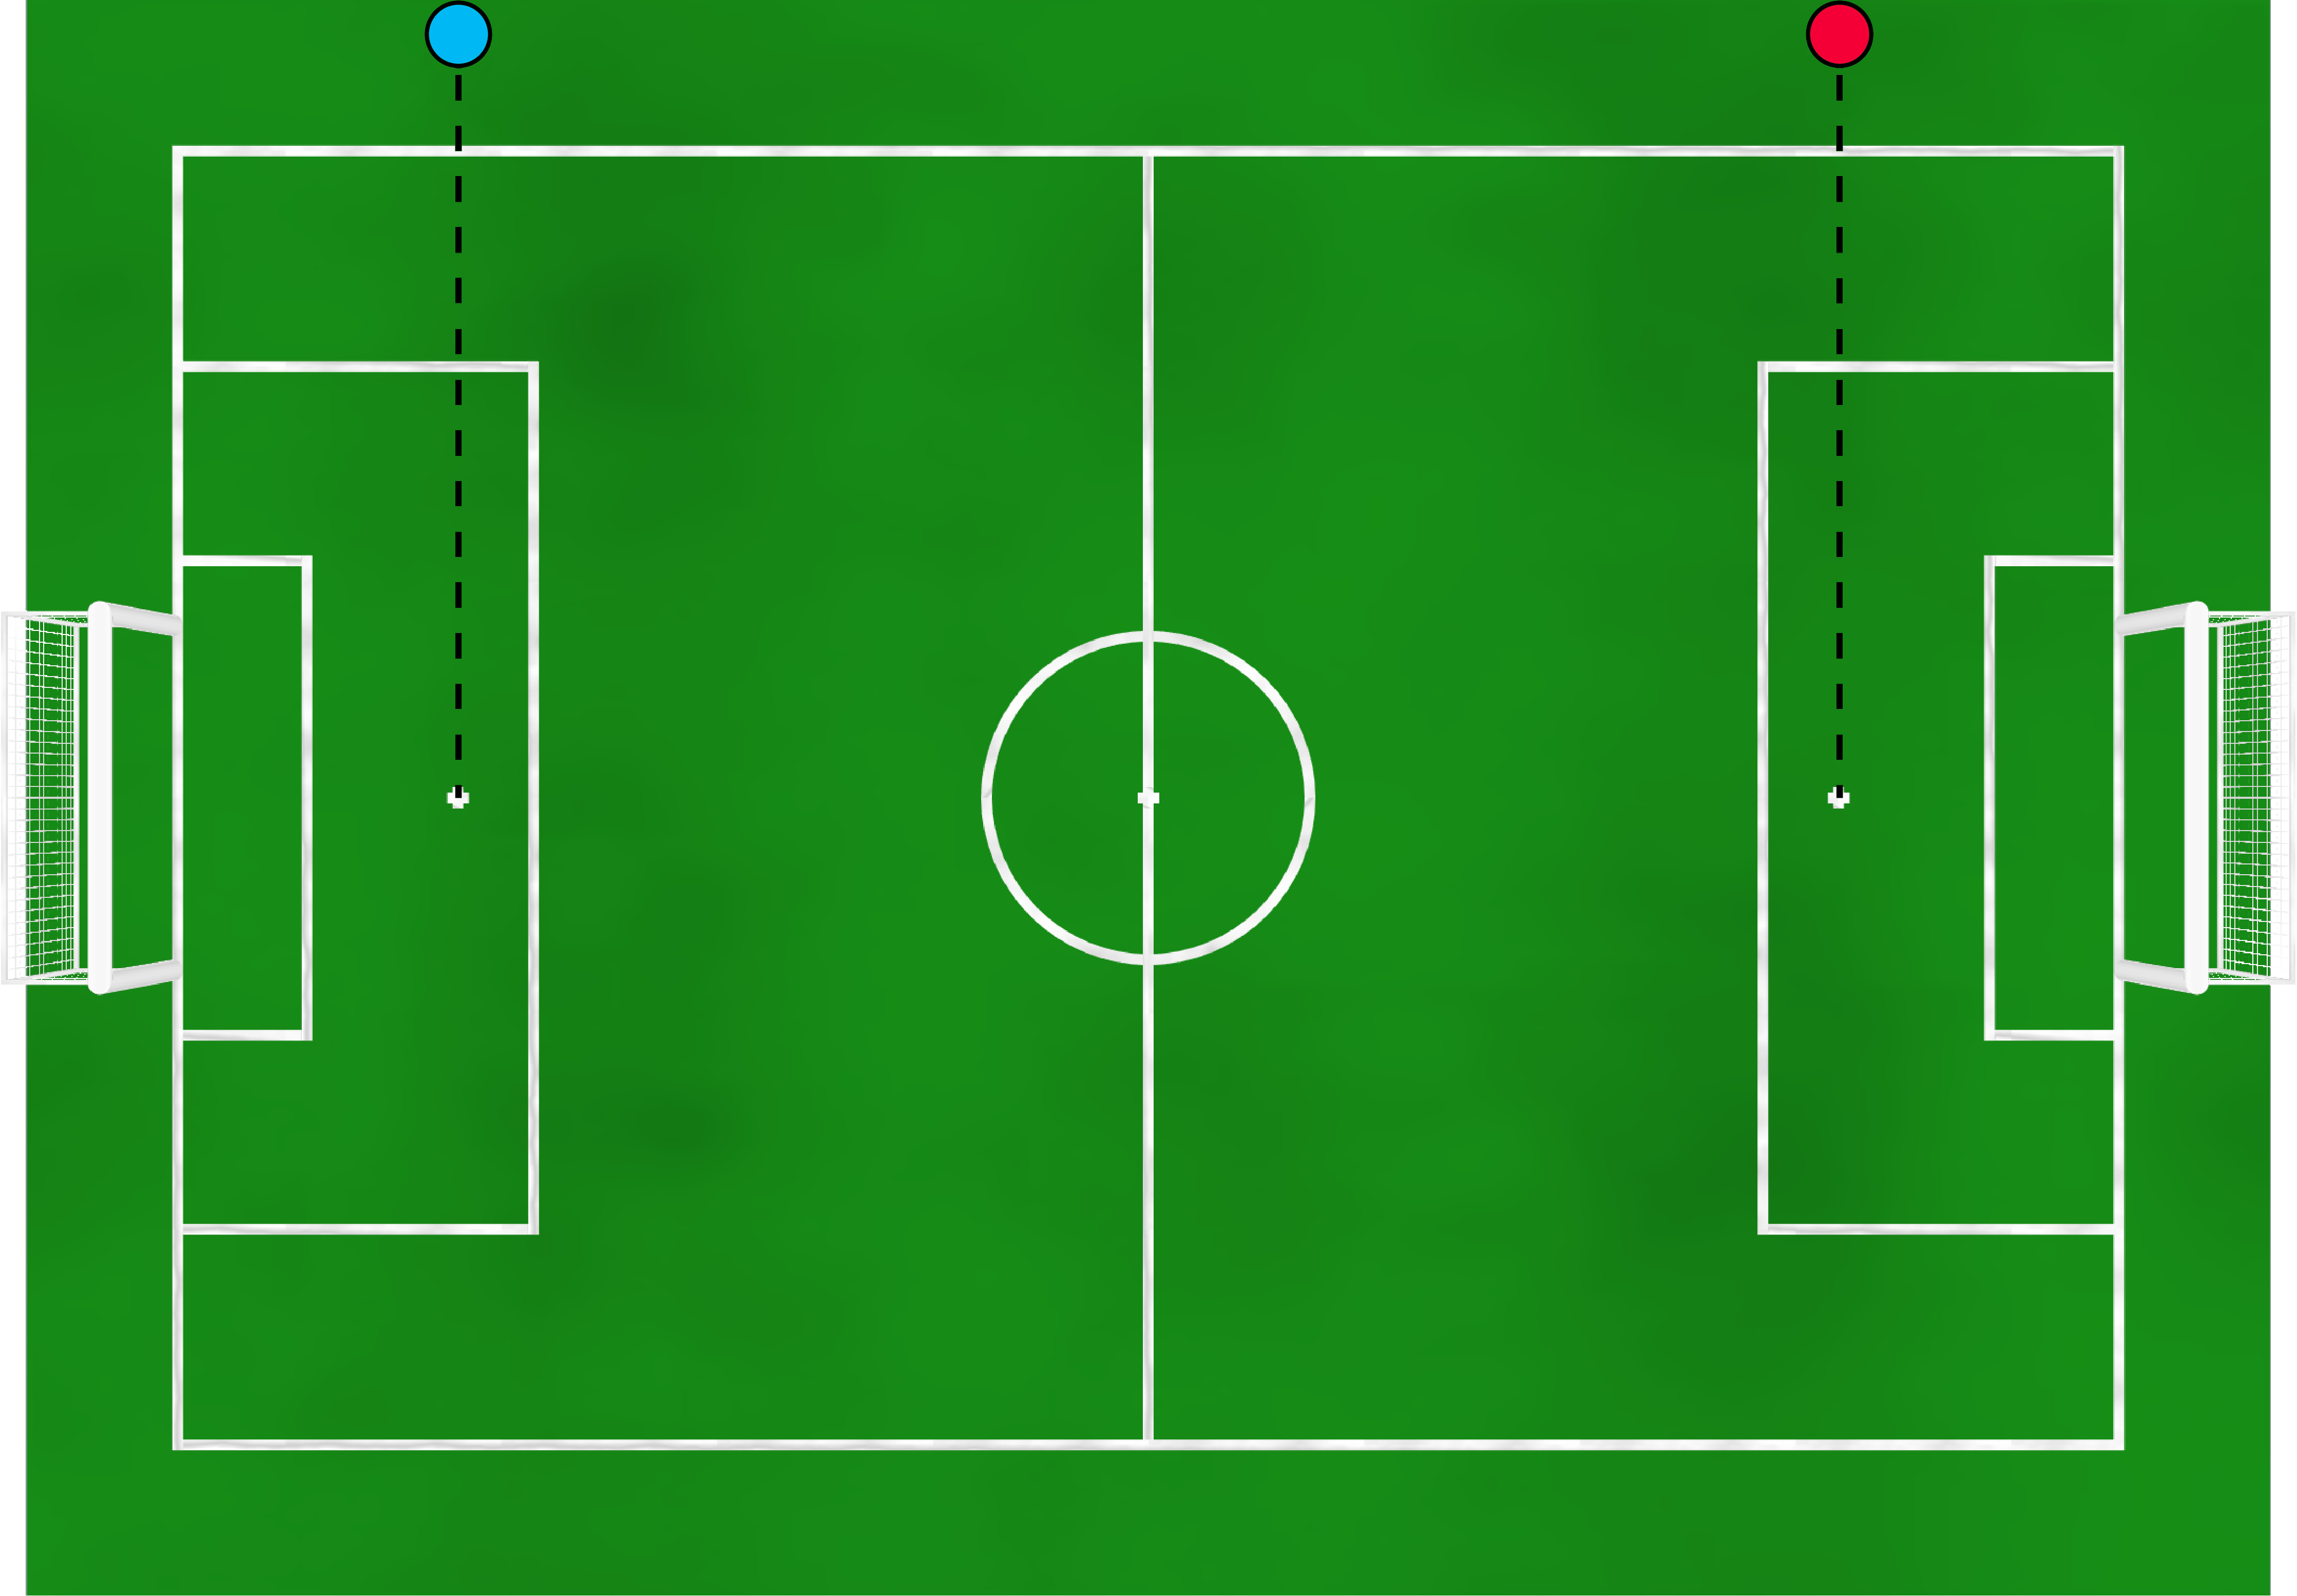
\includegraphics[width=\columnwidth]{figs/penalty_re-entry_points_2024.png}}
    \caption{For robots coming back from a standard removal penalty, re-entry points are in line with or around the penalty mark in their own half, but always where the robots were placed at the beginning of the penalty.}
    \label{fig:penalty_re-entry_points}
\end{figure}

After the penalty time elapses, the GameController operator will remove the penalty from the penalized robot, enabling it to autonomously re-enter the game without requiring additional intervention from the referees.

\subsection{Forbidden Actions}

The following actions are forbidden, but not treated as penalties.
Each forbidden action specifies the actions to be taken by the referees.

\subsubsection{Manual Interaction by Team Members}

Manual interaction with the robots, either directly or via some communications mechanism, is not permitted.
Team members can only touch one of their robots when an assistant referee hands it over to them after a ``Request for Pick-up''.

\subsubsection{Damage to the Field}
\label{sec:damage}

A robot that damages the field, or poses a threat to spectator safety, will be removed from the field for the remainder of the game.

\subsection{Illegal Positioning}
\label{sec:illegal_positioning}

A robot penalized under illegal position has the ``Illegal Position'' penalty applied.
Illegally positioned robots are subject to the standard removal penalty (\cf \cref{sec:removal_penalty}).
The head referee will call ``Illegal Position  \textless robot\textgreater''.
Referees may interchange ``Illegal Position'' with ``Illegal Defender'' to help with clarity.

Illegal positions are descried below.

For simplicity, Illegal Positioning penalties during the \texttt{set} state (for kick-off or a penalty kick) do not count towards the incremental penalty count.

Refer to \cref{sec:inside_outside} for the definition of \textit{inside/outside} of a region of the field.

\subsubsection{Before and During Kick-off}
\label{sec:ip_kick_off}

If a robot violates the positioning restrictions made in \cref{sec:kick-off} at the time the \texttt{set} state starts, it will be penalized and removed for \qty{15}{\second}.
If a robot enters the areas of the other team before the ball is in play, it will be penalized and removed according to the standard removal penalty.

\subsubsection{Own Goal Area}
\label{sec:ip_own_goal_area}

During the \texttt{set} and \texttt{playing} states, at most \textit{three} players can be within their own goal area at the same time.

A robot is within the goal area if any part of its body is touching the ground inside the goal area or touching one of its lines.
The penalty is applied when any additional players enter the area in \texttt{playing}, or to the excessive players closest to the border of the goal area in \texttt{set}.
Note that if a player is pushed into the goal area by an opponent, this robot will not be subject to removal, unless it fails to exit the area within \qty{5}{\second} (or \qty{5}{\second} after getting up if the pushing led to falling).

If an illegal defender kicks an own goal, the goal is scored for the opponent.
If there is any doubt about whether a goal should count (\eg the illegal defender infraction is called, but the robot scores the own goal immediately afterwards, before it is removed) then the decision shall be against the infringing robot.

\subsubsection{Defender Encroachment During Free Kick}
\label{sec:ip_free_kick}

If a robot of the defensive team enters or does not attempt to leave the circular area with \qty{\FreeKickRadius}{\metre} radius around the ball after a free kick (\cf \cref{sec:free_kick}) was called, ``Illegal Position'' is called.
Note that the referee should not look for exact distances and rather penalize only those robots who clearly violate this rule.
As a guideline, the robots of the defensive team should clear the ball within \qty{10}{\second}.

\subsubsection{Penalty Area During Penalty Kick}
\label{sec:ip_penalty_kick}

If a robot enters the relevant penalty area during a penalty kick, except for the goalkeeper (defending team) and one robot of the attacking team, ``Illegal Position'' is called.

\subsection{Forbidden Motion}
Robots that begin moving their legs or locomote in any fashion before reaching the specified state in the subsections
will be penalized \textit{in place} on the field for \qty{15}{\second} in \textit{playing}. It's important to note that the penalty duration only counts down during the playing state.
``Forbidden Motion'' penalties do not follow the standard removal procedure, and hence do not count towards the incremental penalty count.
A robot will be moved back to its original position if it has moved significantly before becoming penalized.

\subsubsection{Motion in Standby}
\label{sec:motion_in_standby}

Robots that begin to move during \texttt{standby} (\ie before the head referee does the visual signal).
The head referee will call ``Forbidden Motion in Standby\textless robot\textgreater''.
Note that responding to any false signal of any fashion will result in this penalty.

\subsubsection{Motion in Set}
\label{sec:motion_in_set}

Robots that begin moving during \texttt{set} (\ie before the head referee blows the whistle).
The head referee will call ``Forbidden Motion in Set \textless robot\textgreater''.
Note that responding to a whistle on another field will result in this penalty.

\subsection{Fallen or Inactive Robots}
\label{sec:fallenrobots}

If a robot falls during the game, it should start executing a get-up action within \qty{5}{\second}.
If it does not commence a get-up action within \qty{5}{\second}, it will be penalized and removed for \qty{45}{\second}.
A fallen robot which is unable to autonomously stand up within 2 attempts, or 3 if disturbed externally during the first two attempts, will be penalized and removed for \qty{45}{\second}.
In both cases, the head referee will call ``Fallen Robot  \textless robot\textgreater''.
The goalkeeper, inside its own penalty area, is the only robot permitted to `dive' (that is deliberately falling in a way that might cause its torso, arms, or hands) to intercept the ball.
In all other cases, the robot should remain upright---that is, supported by its feet.

A robot that has ceased activity for \qty{10}{\second} or has turned off will be removed and penalized for \qty{45}{\second}.
The head referee will call ``Inactive Robot \textless robot\textgreater''.
A robot is active if it performs at least one of the following:
\begin{enumerate}
  \item The robot walks in any direction, or turns.
  \item The robot searches for the ball, or is looking at the ball.
\end{enumerate}

Fallen/Inactive Robot penalties do not follow the standard removal procedure, and hence do not count towards the incremental penalty count.

\paragraph{Note:} The intention of this rule is not to penalize robots simply for being stationary---provided they are not `asleep' and have not `crashed'.

\subsection{Local Game Stuck}
\label{sec:pen_local_game_stuck}

When Local Game Stuck is called, the nearest robot to the ball will be penalized and removed for \qty{45}{\second}.
Local Game Stuck penalties do not follow the standard removal procedure, and hence do not count towards the incremental penalty count.

\subsection{Ball Holding}
\label{sec:ball_holding}

The goalkeeper is allowed to hold the ball for up to \qty{10}{\second} as long as it has one foot inside in its own penalty area.
In all other cases (except those noted in \cref{sec:situations_no_ball_holding}), robots are allowed to hold the ball for up to \qty{3}{\second}.
Holding the ball for longer than this is not allowed.
The head referee will call ``Ball Holding \textless robot\textgreater'', and the robot removed under the standard removal penalty.
The ball should be removed from the possession of the robot and placed where the penalty occurred.
If the robot that held the ball has moved the ball before the robot can be removed, the ball shall be replaced where the penalty occurred.
This applies to accidental goals.

\textbf{Example.} A robot holds the ball, and before the referees can remove the robot, it shoots the ball into the goal.
The goal will not be counted, and the ball will be replaced where the penalty occurred.

A robot must leave enough open space around the ball.
The occupation of the ball is judged using the convex hull of the projection of the robot's body onto the ground.
``Enough open space'' means that at least the half of the ball is not covered by the convex hull.
It is not important whether the robot actually touches the ball.

\begin{figure}[t]
  \centerline{\begin{tabular}{ll}
  a) & b) \\
  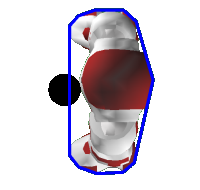
\includegraphics[scale=0.7]{figs/holding1} &
  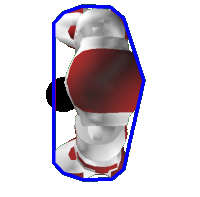
\includegraphics[scale=0.7]{figs/holding4}
  \end{tabular}}

  \caption{Examples for ``Ball Holding''. The black circle is the ball and the blue polygon visualizes the convex hull of the robot's projection onto the ground. Situation a) is legal, whereas b) violates the rule.}
  \label{fig:holding}
\end{figure}

Intentional continual holding is prohibited even if each individual holding time does not continue for up to the time limit.
In general, robots should release the ball for approximately as long as they were holding it to reset the clock.
Without a sufficient release, the continual holding is regarded as a continuous hold from the very beginning and the holding rule is strictly applied.

\subsubsection{Exceptions to the Ball Holding Rules}
\label{sec:situations_no_ball_holding}

The following define situations where ball holding does not apply:
\begin{enumerate}
  \item Ball holding may not occur when the ball becomes stuck between a robot's legs.
    In such a situation, the head referee should call `clear ball' and an assistant referee should remove the ball and place the ball approximately where it was before it became stuck.
  \item Ball holding may not occur when a robot falls on a ball.
    The robot will either get up and hence free the ball, or the robot should be removed under the Fallen Robot rule.
\end{enumerate}

\subsection{Player Stance}
\label{sec:player_stance}

Robots must not maintain a stance wider than the width of their shoulders by more than one robot hand width on each side for longer than \qty{10}{\second}. This duration should be adequate for a robot gesture. Staying in a wide stance for longer than \qty{10}{\second} will result in the standard removal penalty.

This rule applies to upright robots only, \ie robots that are supported by their feet.
Other cases are handled by the fallen robot rule (\cf~\cref{sec:fallenrobots}).

\subsection{Player Pushing}
\label{sec:player_pushing}

% basic definition of pushing
\emph{Pushing} is a direct or indirect forceful contact with any other opponent robot, \ie, enough to destabilize it, and is not allowed.
In the following, exceptions to this rule are specified in more detail.
The head referee will call ``Pushing \textless robot\textgreater''.

If the ball moves significantly as the result of pushing, then it should be replaced to where it was at the time of the infraction.

A \textbf{Pushing Free Kick}, see~\cref{sec:free_kick}, is awarded against the robot penalized for pushing
\begin{itemize}
  \item[1.] if the robot is in an approximately \qty{0.5}{\metre} radius around the ball and
  \item[2.] if the pushed robot was \textbf{not} inside the penalty area of the pushing robot.
\end{itemize}

A \textbf{Penalty Kick}, see~\cref{sec:penalty_kick}, is awarded against the robot penalized for pushing
\begin{itemize}
  \item[1.] if the robot is in an approximately \qty{0.5}{\metre} radius around the ball and
  \item[2.] if the pushed robot was inside the penalty area of the pushing robot.
\end{itemize}

The following exceptions define situations where pushing does not apply:
\begin{itemize}
  \item Pushing may occur \textbf{only} between players of different teams.
  \item A stationary robot cannot be penalized for pushing, including a robot that is kicking, provided that the ball was close enough where a kick could have succeeded at the start of the kick motion.
  \item A robot currently getting up cannot be penalized for pushing.
  \item The goalkeeper cannot be penalized for pushing while looking at or chasing the ball in its own penalty area.
  \item Front to front contact between robots with the ball between them does not constitute pushing.
  \item Any robot proceeding to the ball whose side (\ie arm, shoulder etc.) makes contact with another robot cannot be called for pushing, even if the second robot is not proceeding to the ball.
  \item A robot pushed by another robot cannot simultaneously be called for pushing itself.
    Only the robot, who initially pushed the other robot, will be called for pushing.
\end{itemize}

\subsection{Playing With Arms/Hands}
\label{sec:hand_ball}

Playing with arms/hands occurs when a field player or a goalkeeper outside its own penalty area moves its arms/hands to touch the ball (except during a fall or get-up).
The goalkeeper is allowed to touch the ball with its arms/hands while it is within its own penalty area.
A robot playing with arms/hands will be subject to the standard removal penalty and the ball will be replaced at the point where it contacted the arms/hands of the offending robot.
If an own goal is scored as a result, the goal should count and the player should not be penalized.

Accidental playing with arms/hands when a robot falls or executes a get-up routine will not be penalized.
If the ball goes out of play in this case, normal kick-in rules will apply (\cf \cref{sec:kick_in}).
However, goals (except for own goals) resulting from a ball contact with the arms/hands during a fall or get-up do not count and result in a Goal Kick (\cf \cref{sec:free_kick}) as if the ball went over the goal line next to the goal.

\subsection{Leaving the Field}
\label{sec:leaving_field}

A robot that intends to leave the \qty{\TotalWidth}{\metre} $\times$ \qty{\TotalLength}{\metre} carpeted area will be subject to the standard removal penalty (\cf \cref{sec:removal_penalty}).
The head referee will call ``Leaving the Field \textless robot\textgreater''.

Additionally, a robot will also be subject to the standard removal penalty, when:
\begin{itemize}
  \item The robot walks into the goalposts or goal net for more than \qty{5}{\second}, this includes robots that are stuck on the goalposts and unable to free themselves.
  \item The robot's fingers become entangled in the net (without any time constraint).
\end{itemize}

\subsection{Jamming}
\label{sec:jamming}

During a match, any robot shall never jam the communication and the sensor systems of the opponents:
\begin{description}
  \item[Wireless communication.] Each robot is only allowed to send a limited number of UDP messages that have to comply with a predefined format (\cf \cref{sec:wireless}).
    If a robot uses a different protocol or sends too much data in a game, penalties will apply.
    If a team violates this rule in multiple games, disqualification from the tournament (including all technical challenges and side competitions) as well as an entry in the penalty list will be the consequence.
    Except for the wireless cards and the access points provided by the organizers of the competition, nobody close to the field is allowed using \qty{2.4}{\giga\hertz} or \qty{5}{\giga\hertz} radio equipment (including cellular phones and/or Bluetooth devices).
  \item[Whistle interference.] Both the teams and the audience shall avoid intentionally confusing the robots by producing similar sounds to the game whistle.
  \item[Acoustic communication.] If acoustic communication is used by both teams, they shall negotiate before the match how they can reduce interference.
    If only one team uses acoustic communication, the robots of the other team shall avoid producing any sound.
    In addition, both the teams and the audience shall avoid intentionally confusing the robots by producing similar sounds to those used for communication.
  \item[Infrared communication.] If infrared communication is used by both teams, they shall negotiate before the match how they can reduce interference (if at all).
    Both the teams and the audience shall avoid confusing the robots by producing similar infrared signals to those used for communication.
  \item[Visual perception.] The use of flashlights is not allowed during the games.
    However, flash photography from the audience is allowable as long as the head referee believes the purpose of the flash is not to jam any of the robots.
\end{description}

\newpage

% !TeX root = ../SPL-Rules.tex
% !TeX spellcheck = en_US
\section{Judgment}
\label{sec:judgment}

The referees are the only persons permitted on the carpeted area (\ie the field and the border area).

\subsection{Head Referee}
\label{sec:head_referee}

The head referee is in charge of the game. Any decision of the head referee is valid. The head referee's decision is final and can not be changed afterwards, even by video proof. There is no discussion about decisions during the game, neither between the assistant referees and the head referee, nor between the audience or the teams and the head referee.

The head referee announces decisions by a clear loud call, and (as required) whistle sound.
The whistle, or where there is no whistle the first verbal word of the referees calls, defines the point in time at which the decision is made.
The referees should make efforts to use consistent and clear calls, and it is preferable for referees to use the calls as specified in these rules\footnote{The calls specified in these rules are detailed in English. With the agreement of the teams, the referees may use suitable calls in any language. The exception to this are technical challenge(s) that depends on the calls as specified.}
The intention of specifying the referee calls is for clarity and consistency across games.

Where a whistle is required, the head referee first whistles and then announces the reason for the whistle.
The head referee may choose to use any normal sports whistle.
Each whistle sound should be short and not too loud as to interfere with other fields and simultaneous games.
The head referee must \textit{only} sound the whistle in circumstances described in these rules.
There are three circumstances when the whistle is sounded, kick-off~(\cf \cref{sec:kick-off}), a goal~(\cf \cref{sec:goal}), and ending a half of gameplay~(\cf \cref{sec:game_struct}).

The head referee should avoid handling the ball (except for placing a ball for kick-off), and avoid handling the robots.
Their duty is to monitor and adjudicate the game.
The head referee should only handle robots and the ball if absolutely necessary to expedite gameplay or removal of penalized robots, where the assistant referees are otherwise occupied or too far away.

The head referee should be equipped with a suitable referee jersey, whistle, coin, and black or dark-blue socks.

The head referee may decide at any point before or during a game to relocate any objects around the field, or direct persons to another position around the field.

\subsection{Assistant Referees}
\label{sec:assist_referee}
The two assistant referees handle the robots and the ball. They take the robots out when they are penalized, and they put the robots in again. If a team requests to pick up a robot, an assistant referee will pick it up and give it to one of the team members once the head referee approves. An assistant referee will also put the robot back on the field. An assistant referee will also replace the ball when it goes off the field or becomes stuck between a players feet.

The assistant referees can \textit{indicate} violations against the rules committed by robots to the head referee, so that the head referee can decide whether to penalize a certain robot or not. Assistant referees should only enter the field to execute a decision made by the main referee. They should not prevent robots from falling during the game.

The assistant referees should be equipped with a suitable referee jersey, and black or dark-blue socks.

\subsection{GameController Operator}
\label{sec:gameControllerOp}
The operator of the GameController sits at a PC outside the playing area.
As with the head referee, the operator should make efforts to use consistent and clear calls.
They will signal any change in the game state to the robots via the wireless as they are announced by the head referee.
Note that for both kick-offs and goals, the moment of whistling is determining, not the verbal announcement of the head referee.
The operator will also inform the assistant referees when a timed penalty is over and a robot has to be placed back on the field.
They should announce when the ball is in play on kick-off by stating ``Ball Free'', if the \qty{\KickOffBallFreeTime}{\second} time period has elapsed in the playing state.
They are also responsible for keeping the time of each half (\ie, they stop the clock after a goal or game stuck, and continues it at the kick-off\footnote{The clock may not be stopped during the preliminaries.}).
They should count aloud the remaining seconds in a half once the time remaining is \qty{5}{\second} or less.
Finally, they should repeat the calls of the head referee to make sure it was heard correctly.

\subsection{Referee--Team communication}
\label{sec:referee_team_communiation}
Both teams send a representative called team captain to the field \qty{10}{\minute} before their match starts. This time should be used for welcome each other, choose for side and kick-off (see~\cref{sec:field_side_and_initial_kickoff}) and discuss match related topics.

During the match only the team captains are allowed to communicate with the head referee. Only the team captains and two more people per team are allowed to stay next to the game controller tables. The rest of the team locates themselves around the other sides of the field if they want to watch the match. This allows the referees easier communication with the team and the game controller operator gets less disturbed.

After the match the teams thank the referees for their duty.

During all phases of the match teams and referees are communicating with respect to each other.

\subsection{Referees During the Match}

The head referee and the assistant referees should wear socks \emph{of black or dark blue color} and avoid reserved colors (white and green). They may enter the field in particular situations, \eg, to remove a robot when applying a penalty. They should avoid interfering with the robots as much as possible.

\newpage


\appendix

% !TeX root = ../SPL-Rules.tex
% !TeX spellcheck = en_US
\section{The Official RoboCup Competition Rules}
\label{sec:comRules}
This section contains rules that are not directly relevant for games and that may not apply at local opens.  However, these rules will be upheld at the yearly international RoboCup competition.

\subsection{Qualification Procedure and Code Usage}
\label{sec:qualification_procedure_codeuse}

The qualification procedure as well as the corresponding deadlines will be announced by the Technical Committee before qualification applications are accepted.

The RoboCup Standard Platform League offers unique possibilities to use code from other teams. In spirit of the RoboCup every team is generally allowed to use code from other teams to push the league further with their own research.
This use must be cited.
However, every participant of RoboCup \textbf{\textit{has a duty}} to contribute to the league.

To qualify, every team must make at least \textit{novel contribution} within their soccer software.
A team must have made at least one contribution within the last \NovelContributionTime.
Contributions outside of this period are no longer considered sufficiently novel and a team must make at least one \textit{new} contribution.
It is also \textit{mandatory} for a team to use their novel contribution in all competition games.
A novel contribution is:
\begin{itemize}
  \item Research publishable contribution to a \textit{game critical module}
  \item Complete replacement of a \textit{game critical module}, with original software. This may not necessarily be research publishable, but must be of equivalent scale and quality to research publishable work.
\end{itemize}

It is not a novel contribution to replace a module with code copied from another source, or to simply train a machine-learning model released by another team using new data.

As of the \RCYear competition, the following are recognized as game critical modules:
Ball detection, Robot detection, Robot vision (not otherwise listed), Localization, Walk/Kick engine, Dynamic stabilization, Behavior Architecture, \& Distribution computation, Whistle detection.

As of the \RCYear competition, the following are \textit{not} recognized as sufficiently game critical (even if the ability to play soccer depends on these):
Hand-written Soccer Behaviors, Natural Language detection, \& Robot and GC Communication.

In their qualification application, teams may petition the technical committee to recognize other novel contributions not listed here.
Additionally, a team that has participated at RoboCup for at least \NovelContributionTime consecutively may petition the technical committee to recognize contributions to non-game critical modules, such as developing infrastructure for the league\footnote{However, the technical committee should balance whether a team is continuing to use their own software in games.}.
A team may also petition for the technical committee to reconsider the list of game critical and non-game critical modules.
Successful petitions will be public ally announced to the league for transparency.
%For example, a team may petition and provide evidence that their work on the whistle detection is substantial and game critical, thus satisfying the requirements of a novel contribution.

If a team that is otherwise eligible for qualification cannot provide sufficient evidence of the required contributions by the deadline for applications, then that team may be qualified for RoboCup \textit{on probation}.
In this case, the team must provide evidence of the required contributions to become \textit{fully} qualified by the registration deadline of the RoboCup event.
If no suitable evidence is provided, the team's probationary qualification will lapse.

Every applicant must also bring a poster containing the team's contribution, focused on the current year, to the RoboCup event to share their contributions with the other teams.

Failure to meet any of these requirements will result in a qualification penalty for subsequent years.

\subsection{Champions Cup and Challenge Shield}
\label{sec:cc_and_cs}

Two separate competitions are played: the champions cup for the strongest teams and the challenge shield for all other teams.
Teams are assigned to one of the competitions during the application phase, considering their preference, ability and organizational aspects.
Matches in the champions cup are played with 7 players on each team, while the challenge shield is played with 5 players on each team (\cf~\cref{sec:robot_players}).

\subsection{Game Structure}

The clock stops during stoppages of play (such as \texttt{ready} and \texttt{set} state after goals) from the quarter-finals onward.  In round robin pool play, a game can finish in a draw as no penalty shoot-out will follow. In the promotion round, intermediate round, quarter finals, semi finals, 3rd place or final, a game that ends in a draw will be followed by a penalty shoot-out (see \cref{sec:penalty_shoot-out}).

\subsection{Competition Mode}

Depending on the number of participating teams, the OC and TC create a competition table. The following modes can be selected:

\begin{itemize}
  \item Group games, with or without intermediate rounds, with concluding knock-out phase
  \item Double elimination system
  \item Swiss tournament system
  \item Swiss tournament system with concluding knock-out phase.
\end{itemize}

All teams participating in the competition are initially ranked using the Glicko system\footnote{\url{http://www.glicko.net/glicko/glicko.pdf}} based on all available results from previous official RoboCup tournaments. (New teams will be ranked equally below all previously competing teams. Teams that participated previously but did not participate in the previous year will be ranked above new teams but below teams that competed in the previous year.)

The OC will announce two weeks before a competition:

\begin{itemize}
  \item Competition mode and which competition rules will be applied
  \item Initial ranking of participating teams
  \item How to determine the overall winner and the ranking of the technical challenges
  \item Pre-qualification rules.
\end{itemize}

\subsection{Referee Selection and Requirements}
\label{sec:refSelection}
During pool play, the games will be refereed by members of teams from a different pool.

Each team has to referee a number of games. A schedule will be released specifying the games for which each team is required to provide two referees. Referees should report to the appropriate field at least ten minutes before the game is scheduled to start.

If a team fails to provide two referees for a game in which they are scheduled to provide referees, it will be noted by the organizing committee and recorded as a \textbf{qualification penalty} (\cref{sec:qualificationPenalties}).

For each of the games, a team will be required either to provide the head referee and the operator of the GameController, or the two assistant referees.  The two teams assigned to referee a game shall decide among themselves which roles each team will fulfill. Note, however, that the head referee and the GameController should always be from the same team.

A team may swap their scheduled refereeing duties with another team, but the team listed on the referee schedule will be held accountable if referees fail to appear for a game they are scheduled to referee.

The requirement to referee may be an extreme hardship for extremely small teams.  If a team believes providing two referees for games will be an extreme hardship, they must send an email explaining their situation to the Organizing Committee and Technical Committee at least two weeks before the first set up day of the competition.  The Organizing and Technical Committees will then consider the request and attempt to find an acceptable solution.

Referees must have good knowledge of the rules as applied in the tournament, and the operator of the GameController must be experienced in using that software. Referees and the GameController should be selected among the more senior members of a team, and preferably have prior experience with games in the RoboCup Standard Platform league.

In each game, each of the teams playing shall be able to veto one and only one eligible referee with no reason required. The veto must be delivered before the start of the \texttt{ready} phase or during a stoppage of play.

\subsection{Rules for Forfeiting}
\label{sec:forfeit}

Teams who do not make a good faith effort to participate in a scheduled game are considered to forfeit the game.

If a team notifies the technical committee that they wish to forfeit less than two hours before their scheduled game time, simply fails to show up for their game, or decides during their game that they wish to forfeit, then the opposing team will play the match against an empty field.  However, any own goals will not be scored.  Hence, after an opponent forfeits, the team playing against an empty field cannot do worse than they were doing at the time the opponent decided to forfeit.  Teams may choose to forfeit at any stoppage of play.  However, once a forfeit is announced, they may not reverse this decision.

If a team notifies the technical committee that they wish to forfeit at least two hours before their schedule game time, the following procedure will be followed.

\begin{itemize}
  \item If a team chooses to forfeit a match in the round robin games the other team plays the match against an empty field.  However, any own goals will not be scored.
  \item If a team chooses to forfeit in a knock-out game it gets replaced by the next best qualified team, \ie the team it kicked out or left behind in the round robins.
\end{itemize}

Note that there are a few unlikely cases that are not covered by these rules.  If a situation is not covered by these rules, the technical committee and the organizing committee will work together to make a decision.

Any forfeit will result in a qualification penalty being recorded (\cf \cref{sec:qualificationPenalties}) but the circumstances of the forfeit will affect the severity of the offense and the impact on future qualification.

\subsection{Source Code Releases}
\label{sec:source_code_releases}

All teams that have participated in RoboCup must subsequently release code from that year's codebase.
The code must be licensed such that other RoboCup participants can use it, although the license may place conditions on its use.
The preferred type of release is the full source code of the software that was running in the team's last game at RoboCup.
In case this is not possible (\eg due to legal reasons), it is required that at least the source code related to the novel contributions (as given during the qualification process) is published.
Participation in technical challenges may come with additional requirements on the amount of components to be released.

The source code must be published and its availability announced on the SPL mailing list (\url{robocup-nao@lists.robocup.org}) by \DTMdate{\CodeReleaseAnnouncementDate}.
Failing to publish source code by the deadline will result in a qualification penalty being recorded (\cf~\cref{sec:qualificationPenalties}).

\subsection{Subsequent Year Pre-qualification Procedure}
\label{sec:preQual}

Teams may become pre-qualified for the subsequent year's competition by fulfilling criteria set two weeks before the competition.
Pre-qualified teams do not compete with other teams' applications during the qualification process.
However, the call for participation for the subsequent year's competition may set additional formal requirements that must be fulfilled in order to remain pre-qualified.

\subsection{Qualification Penalties}
\label{sec:qualificationPenalties}

There are a number of offenses which lead to qualification penalties being recorded against a team. These are as follows:
\begin{itemize}
    \item Withdrawing from RoboCup after the final commitment deadline
    \item Failing to referee when assigned (\cref{sec:refSelection})
    \item Forfeiting a game (\cref{sec:forfeit})
    \item Failing to publish source code by the deadline (\cref{sec:source_code_releases})
\end{itemize}

A team cannot be pre-qualified for RoboCup in the year following a qualification penalty. Furthermore, a qualification penalty is considered by the Technical Committee when reviewing applications and will negatively affect the assessment of a team's application. Multiple penalties accumulate and will result in an even more negative assessment of a team's application. Qualification penalties are considered for a period of three years following the offense.

Whenever a qualification penalty is recorded, all relevant details including any possible mitigating circumstances are also recorded and these will also inform the assessment of a team's application.

\subsection{Disqualification During Competition}
\label{sec:disqualification_during_comp}

A team may be disqualified during the RoboCup competition for:
\begin{itemize}
  \item A serious violation of the terms of a team's qualification
  \item Gaining a Qualification Penalty during the course of the competition~(\cf \cref{sec:qualificationPenalties})
  \item A serious breach of ethics, or serious behavior unbecoming of participants of RoboCup.
\end{itemize}

\textbf{Example.} A team promises to use their novel contribution in RoboCup games, but fails to do so.
Alternatively, a team deliberately misleads the technical committee about the novelty of their work and/or their contribution to the league, such that they are deemed to have copied another team.

A team can \textit{only} be disqualified by a decision of the \textit{Board of Trustees of the RoboCup Federation}.
The RoboCup Soccer SPL executive must petition the board in writing at their soonest possible availability.
The executive must simultaneously inform the relevant team of the petition in writing.

A disqualified team automatically forfeits all games~(\cf \cref{sec:forfeit}).
For practicality, the disqualification should not apply \textit{retroactively}.
However, by majority vote of the team leaders, provisions for retroactive disqualification may be made in the fairness of the affected teams.

\newpage

% !TeX root = ../SPL-Rules.tex
% !TeX spellcheck = en_US
\section{Changes From \LastRCYear}

This is a brief non-normative list of rule changes from \LastRCYear to \RCYear:
\begin{itemize}
  \item Teams can be restricted from blocking natural light at the competition (\cf~\cref{sec:lightConditions}).
  \item The Standard Removal Penalty was simplified. Robots will be placed behind the touchline facing towards the field, while penalized (\cf~\cref{sec:removal_penalty}).
  \item The transition from the \texttt{initial} to \texttt{ready} state is announced via visual referee signal and the signal of the GameController is delayed (\cf~\cref{sec:robot_states}).
  \item The rules regarding direct kick goals were tightened for Champions Cup matches. More dynamic ball handling is required to score goals (\cf~\cref{sec:indirect_kick_champions}).
  \item Global Game Stuck was changed with regards of choosing the team that receives kick-off (\cf~\cref{sec:game_stuck:global}).
\end{itemize}

\newpage

\section{Field Technical Drawings}
\label{apx:technical-drawing}
\centerline{\includegraphics[angle=90,origin=c,width=\columnwidth]{figs/field_technical.pdf}}

\clearpage
\centerline{\includegraphics[angle=90,origin=c,width=0.5\columnwidth]{figs/field_technical_cc.pdf}}

\centerline{\includegraphics[origin=c,width=0.5\columnwidth]{figs/field_technical_pm.pdf}}

\end{document}
